\section{Signal extraction strategy}
\label{sec:signal_extraction}

% Directory with the transfer factor plots
\newcommand\tfPlotDir{TransferFactors/merged_2023-04-08_vbfhinv_full_analysis_NLO_VJets_09Apr23_thesis_v1}

The largest background contributions from \Zvvjets~and \Wlvjets~processes
are estimated using data from five mutually exclusive control regions (CR), which are described in
Sec.~\ref{sec:event_selection}. These control regions consist of:

\begin{itemize}
  \item $\Wmnjets$ region (Sec.~\ref{sec:selection_cr_1m})
  \item $\Wenjets$ region (Sec.~\ref{sec:selection_cr_1e})
  \item $\Zmmjets$ region (Sec.~\ref{sec:selection_cr_2m})
  \item $\Zeejets$ region (Sec.~\ref{sec:selection_cr_2e})
  \item $\gamma$ + jets region (Sec.~\ref{sec:selection_cr_g})
\end{itemize}

$\Vjets$ yields in the signal region is estimated by performing a simultaenous fit to the data 
in all signal and control regions, as will be explained in detail in Sec.~\ref{subsec:likelihood_fit}.

The remaining backgrounds that contribute to the total event yield in the signal region
are much smaller than those from \Zvvjets~and \Wlvjets~processes, due to the fact that they are
suppressed by kinematic cuts imposed in the VBF signal region (please see Sec.~\ref{subsec:sr_vbf_selection} for the discussion). 
These backgrounds can be summarized as the following: 

\begin{itemize}
    \item QCD multijet events, measured from data using a $\Delta\phi$ extrapolation method~\cite{VBFHinvAnalysisPaper}.
    \item Events from forward HCAL (HF) noise, measured from an orthogonal CR as explained in Sec.~\ref{subsec:hfnoise}.
    \item Top and diboson processes, which are estimated from simulation.
\end{itemize}

\subsection{Binned likelihood fit}
\label{subsec:likelihood_fit}

A binned maximum likelihood fit to the observed data is performed simultaneously across the 
signal and control regions. For each $\mjj$ bin $i$ in every region, the expected yield of $\Vjets$ events
is parametrized as a function of expected strong $\Zvvjets$ yields in the signal region, labeled as
$\kappazi$. This parametrization is done using transfer factors between different
$\Vjets$ processes, as will be explained later in this section. To scale the expected amount of VBF
$\hinv$ signal in the VBF signal region, a signal strength parameter $\mu$ is also introduced to
the fit, and left freely floating. The resulting likelihood function is shown in Eq.~\ref{eq:fit_likelihood_func}.

% A combined likelihood function is constructed representing the Poisson probability to observe the data
% in each $\mjj$ bin, given the expected background yields. This likelihood function consists of
% the product of Poisson probabilities for each $\mjj$ bin in every region (signal region and the 
% five control regions). The likelihood function is presented in Eq.~\ref{eq:fit_likelihood_func}.

% 
% Likelihood from AN
% 

% \begingroup
% \small
% \begin{align}
% \mathcal{L}(\boldsymbol{\mu}^{\Zvv}, \boldsymbol{\mu}, \boldsymbol{\theta}) = &
% \prod_{i} \mathrm{Pois}\left(d_{i} | B_{i}(\boldsymbol{\theta}) + (1+f_{i}(\boldsymbol{\theta})_{\mathrm{QCD}}) \muz_{i} + R^{EW/QCD}_{i} (1+f_{i}(\boldsymbol{\theta})_{\mathrm{EW}}) \muz_{i}+ \boldsymbol{\mu} S_{i}(\boldsymbol{\theta})\right ) \times \nonumber\\
% &\prod_{i} \mathrm{Pois} \left(d^{Z}_{i}|B^{Z}_{i}(\boldsymbol{\theta}) +\frac{\muz_{i} }{R^{Z}_{i} (\boldsymbol{\theta})_{\mathrm{QCD}}} + \frac{\muz_{i} }{R^{Z}_{i} (\boldsymbol{\theta})_{\mathrm{EW}}} \right) \times \nonumber\\
% & \prod_{i} \mathrm{Pois}\left(d^{W}_{i}|B^{W}_{i}(\boldsymbol{\theta}) +\frac{f_{i}(\boldsymbol{\theta})_{\mathrm{QCD}}\,\muz_{i}}{R^{W}_{i}(\boldsymbol{\theta})_{\mathrm{QCD}}}+\frac{f_{i}(\boldsymbol{\theta})_{\mathrm{EW}}\,\muz_{i} }{R^{W}_{i} (\boldsymbol{\theta})_{\mathrm{EW}}} \right) \times \nonumber\\
% & \prod_{i} \mathrm{Pois}\left(d^{\gamma}_{i}|B^{\gamma}_{i}(\boldsymbol{\theta}) +\frac{\muz_{i}}{R^{\gamma}_{i}(\boldsymbol{\theta})_{\mathrm{QCD}}}+\frac{\muz_{i} }{R^{\gamma}_{i} (\boldsymbol{\theta})_{\mathrm{EW}}} \right) \nonumber\\
% \end{align}
% \label{eq:fit_likelihood_func}
% \endgroup

\begin{equation}
  \label{eq:fit_likelihood_func}
  \begin{aligned}
  \mathcal{L} (\mu,\kappaz, \boldsymbol{\theta}) = & \prod_{i} \mathrm{P}\left(d_{i} \Big{|} B_{i}(\boldsymbol{\theta}) + Z_{i}(\kappazi)+W_{i}(\kappazi,\boldsymbol{\theta}) + \mu S_{i}(\boldsymbol{\theta})\right) \\
  %&\prod_{\mathrm{CR}} \left( \prod_{i} \mathrm{P} \left(d^{\mathrm{CR}}_{i} \Big{|} B^{\mathrm{CR}}_{i}(\boldsymbol{\theta}) +\frac{\kappazi }{R^{\mathrm{CR}}_{i} (\boldsymbol{\theta})_{\mathrm{Q}}} + \frac{R^{\PZ}_{i} \kappazi }{R^{\mathrm{CR}}_{i} (\boldsymbol{\theta})_{\mathrm{E}}} \right)\right) \times \prod_{j} \mathrm{P}(\theta_{j}), \\
  & \prod_{\mathrm{CR}} \left( \prod_{i} \mathrm{P} \left(d^{\mathrm{CR}}_{i} \Big{|} B^{\mathrm{CR}}_{i}(\boldsymbol{\theta}) + V_{i}^{\mathrm{CR,strong}}(\kappazi,\boldsymbol{\theta}) + V_{i}^{\mathrm{CR,VBF}}(\kappazi,\boldsymbol{\theta}) \right)\right) \\
   & \prod_{j} \mathrm{P}(\theta_{j}), \\
  Z_{i}(\kappazi) = & (1+Z^{\frac{\mathrm{VBF}}{\mathrm{strong}}}_{i}) \kappazi, \\
  W_{i}(\kappazi,\boldsymbol{\theta}) = & (f^{\mathrm{W/Z,strong}}_{i}(\boldsymbol{\theta}) + Z^{\frac{\mathrm{VBF}}{\mathrm{strong}}}_{i} f^{\mathrm{W/Z,VBF}}_{i}(\boldsymbol{\theta})) \kappazi, \\
  V_{i}^{\mathrm{CR,strong}}(\kappazi,\boldsymbol{\theta}) = & C^{\mathrm{CR,strong}}_{i}(\boldsymbol{\theta}) R^{\mathrm{CR}}_{i}(\boldsymbol{\theta}) \kappazi, \\
  V_{i}^{\mathrm{CR,VBF}}(\kappazi,\boldsymbol{\theta}) = &C^{\mathrm{CR,VBF}}_{i}(\boldsymbol{\theta}) Z^{\frac{\mathrm{VBF}}{\mathrm{strong}}}_{i} R^{\mathrm{CR}}_{i}(\boldsymbol{\theta}) \kappazi, \\
  \end{aligned}
\end{equation}
where ${\mathrm{P}(x|y) = y^{x}e^{-y}/x!}$. $d^{\mathrm{CR}}_{i}$
and $d_{i}$ are the observed number of events in each bin $i$ of
the $\mjj$ distribution in the CRs and SR, respectively. The index $i$ runs
over the $\mjj$ bins in all regions and data taking years (\textit{i.e.,} 2017 and 2018).

In a given bin, $\Vjets$ background yields expected in the SR are
obtained from transfer factors relating the yields in different
CRs to the yields in the SR, denoted as
$R^{\mathrm{CR}}_{i}(\boldsymbol{\theta})$. These transfer factors are 
obtained from simulation. For the single-lepton (dilepton) CRs, the factor
$R^{\mathrm{CR}}_{i}(\boldsymbol{\theta})$ refers to the ratio
of $\Wjets$ ($\Zjets$) yields from the corresponding CR to the SR. In the
photon CR, it refers to the ratio of $\phojets$ to $\Zvvjets$ yields.

In addition, transfer factors are defined between the W ($\gamma$) and
the Z processes, separately for the VBF and strong productions,
denoted as $f^{\mathrm{W/Z,proc}}_{i}(\boldsymbol{\theta})$
($f^{\gamma\mathrm{/Z,proc}}_{i}(\boldsymbol{\theta})$), with
proc denoting the production mode (strong or VBF). Lastly, a transfer factor allows the
relation of the VBF production to the strong production for $\Zvvjets$,
denoted as $Z^{\frac{\mathrm{VBF}}{\mathrm{strong}}}_{i}$. The factors
$C^{\mathrm{CR,strong}}_{i}(\boldsymbol{\theta})$ and
$C^{\mathrm{CR,VBF}}_{i}(\boldsymbol{\theta})$ are dependent on the
CR, with: $C^{(ee,\mu\mu)\mathrm{,proc}}_{i} =
1$, $C^{(e,\mu)\mathrm{,proc}}_{i} =
f^{\mathrm{W/Z,proc}}_{i}(\boldsymbol{\theta})$,
$C^{\gamma\mathrm{,proc}}_{i} =
f^{\gamma\mathrm{/Z,proc}}_{i}(\boldsymbol{\theta})$.

The contributions from subleading backgrounds in each region are
estimated directly from simulation and they are denoted by
$B^{\mathrm{CR}}_{i}(\boldsymbol{\theta})$ in the CRs, and
$B_{i}(\boldsymbol{\theta})$ in the SR. Finally, the likelihood also
includes a signal term in which $S_i$ represents the expected signal
prediction from the sum of the main Higgs production mechanisms
(\ggH, \vbf, \vh, \tth) assuming SM cross sections, while $\mu
= \sigmabr$ denotes the signal strength parameter, also left freely
floating.

Systematic uncertainties are modeled as constrained nuisance
parameters ($\boldsymbol{\theta}$), with a log-normal distribution for
those which affect the overall normalisation of a given process, and
Gaussian priors for those which directly affect the transfer factors,
indicated by $\mathrm{P}(\theta_{j})$ in Eq.~\ref{eq:fit_likelihood_func}.

% 
% Fit description from AN
% 

% The fit is performed simultaneously in the five different control regions and in the signal
% region, for events selected in the VBF category, to estimate the $\Zvvjets$ and $\Wlvjets$ yields
% in each $\mjj$ bin in the signal region.  
% In this likelihood, the expected number of $\Zvvjets$ events in each
% bin of $\mjj$ are the free parameters of the fit ($\boldsymbol{\mu}_{i}^{\Zvv}$). 
% The $\Zvvjets$ and $\Wlvjets$ yields are estimated separately for the
% QCD and EWK components in each $\mjj$ bin. However, the fit is constrained using the $R^{{EWK/QCD}}_{i}$ parameters, which
% represent the ratio between the QCD and EWK components of the $\Zvvjets$ background. This ratio does not have any additional
% uncertainty. The systematic uncertainties ($\boldsymbol{\theta}$) enter the likelihood as 
% additive perturbations to the transfer factors $R^{Z/W/\gamma}_{i}$, and are modeled as Gaussians.

% The parameter $\boldsymbol{\mu}_{i}^{\Zvv}$ represents the yield of the $\Zvvjets$ background in the dijet mass
% bin $i$ in the signal region, and is left freely floating in the fit. The function $f_{i}(\boldsymbol{\theta})$ is the
% transfer factor between the $\Zvvjets$ and $\Wlvjets$ backgrounds in the signal region and represents a constraint between
% these backgrounds. The likelihood also includes the signal region  with $B_{i}$ representing all the backgrounds, $S$
% representing the nominal signal prediction, and $\mu$ being the signal strength parameter also left floating in the fit.

\subsubsection{Transfer factors}
\label{subsubsec:transfer_factors}

Transfer factors, derived from simulation,
are used to link the yields of the $\Zlljets$, $\Wlvjets$ and $\phojets$~processes in the control
regions with the $\Zvvjets$ and $\Wlvjets$ background estimates in the signal region.
These transfer factors are defined as the ratio of expected yields of the target process
in the signal region and the process being measured in the control region. As an example,

\begin{equation}
  R_{i}^{\mathrm{Z}(\mu\mu), \mathrm{strong}}(\boldsymbol{\theta}) = \frac{N_{i,MC}^{\Zvv}}{N_{i,MC}^{\Zmm}}(\boldsymbol{\theta}) \quad ,
  \label{eq:example_tf}
\end{equation}
where $N_{i}$ is the number of events in bin $i$ of the $\mjj$ distribution, 
$R_{i}^{\mathrm{Z}(\mu\mu), \mathrm{strong}}(\boldsymbol{\theta})$ is the transfer factor between the 
strong $\Zmmjets$ process yields in dimuon control region 
and strong $\Zvvjets$ background in the signal region. The transfer factor in
Eq.~\ref{eq:example_tf} allows us to write the strong $\Zmmjets$ yields
in dimuon control region as a function of strong $\Zvvjets$ yields in the signal region
(\textit{i.e.,} $\kappazi$ in Eq.~\ref{eq:fit_likelihood_func}),

\begin{equation}
  % \begin{aligned}
  V_{i}^{\mathrm{Z}(\mu\mu), \mathrm{strong}}(\kappazi,\boldsymbol{\theta}) = R_{i}^{\mathrm{Z}(\mu\mu), \mathrm{strong}}(\boldsymbol{\theta}) \times \kappazi \quad .
  % \end{aligned}
\end{equation}

Other transfer factors are constructed in a similar manner, so that all $V_{i}^{\mathrm{CR,strong}}$ and
$V_{i}^{\mathrm{CR,VBF}}$ can be written as a function of $\kappazi$ and the nuisance parameters, $\boldsymbol{\theta}$. 

Using this transfer factor formalism, $\Zvvjets$ background prediction in the signal region is connected 
to the yields of $\Zmmjets$~and $\Zeejets$~events
in the dilepton control regions. The associated transfer factors account for the differences in the
branching ratio of Z bosons to charged leptons relative to neutrinos and the impact of lepton acceptance and selection
efficiencies. In the case of dielectron events, the transfer factor also takes into account the
difference in the trigger efficiencies. The resulting constraint on the $\Zvvjets$~background from the dilepton
control regions is limited by the statistical uncertainty in the dilepton control regions due to the large
branching fraction difference of the Z boson decays to muons and electrons compared to neutrinos.

Similarly, $\Wlvjets$ background prediction in the signal region is connected to the yields of
$\Wmvjets$ and $\Wevjets$ event yields in single-lepton control regions.
These transfer factors take into account
the impact of lepton acceptances and efficiencies, lepton veto efficiencies, and
the difference in the trigger efficiencies in the case of the single-electron control region.

The transfer factors linking Z and W processes in control regions are validated by comparing the ratio of data in
different control regions to the predicted ratio in simulation. These transfer factors are shown as a function of $\mjj$
in Fig.~\ref{fig:transfer_factors_zoverw}, where the left column shows the results with 2017 data, and the right column
shows the 2018 data. 

\begin{figure}[htbp]
  \centering
    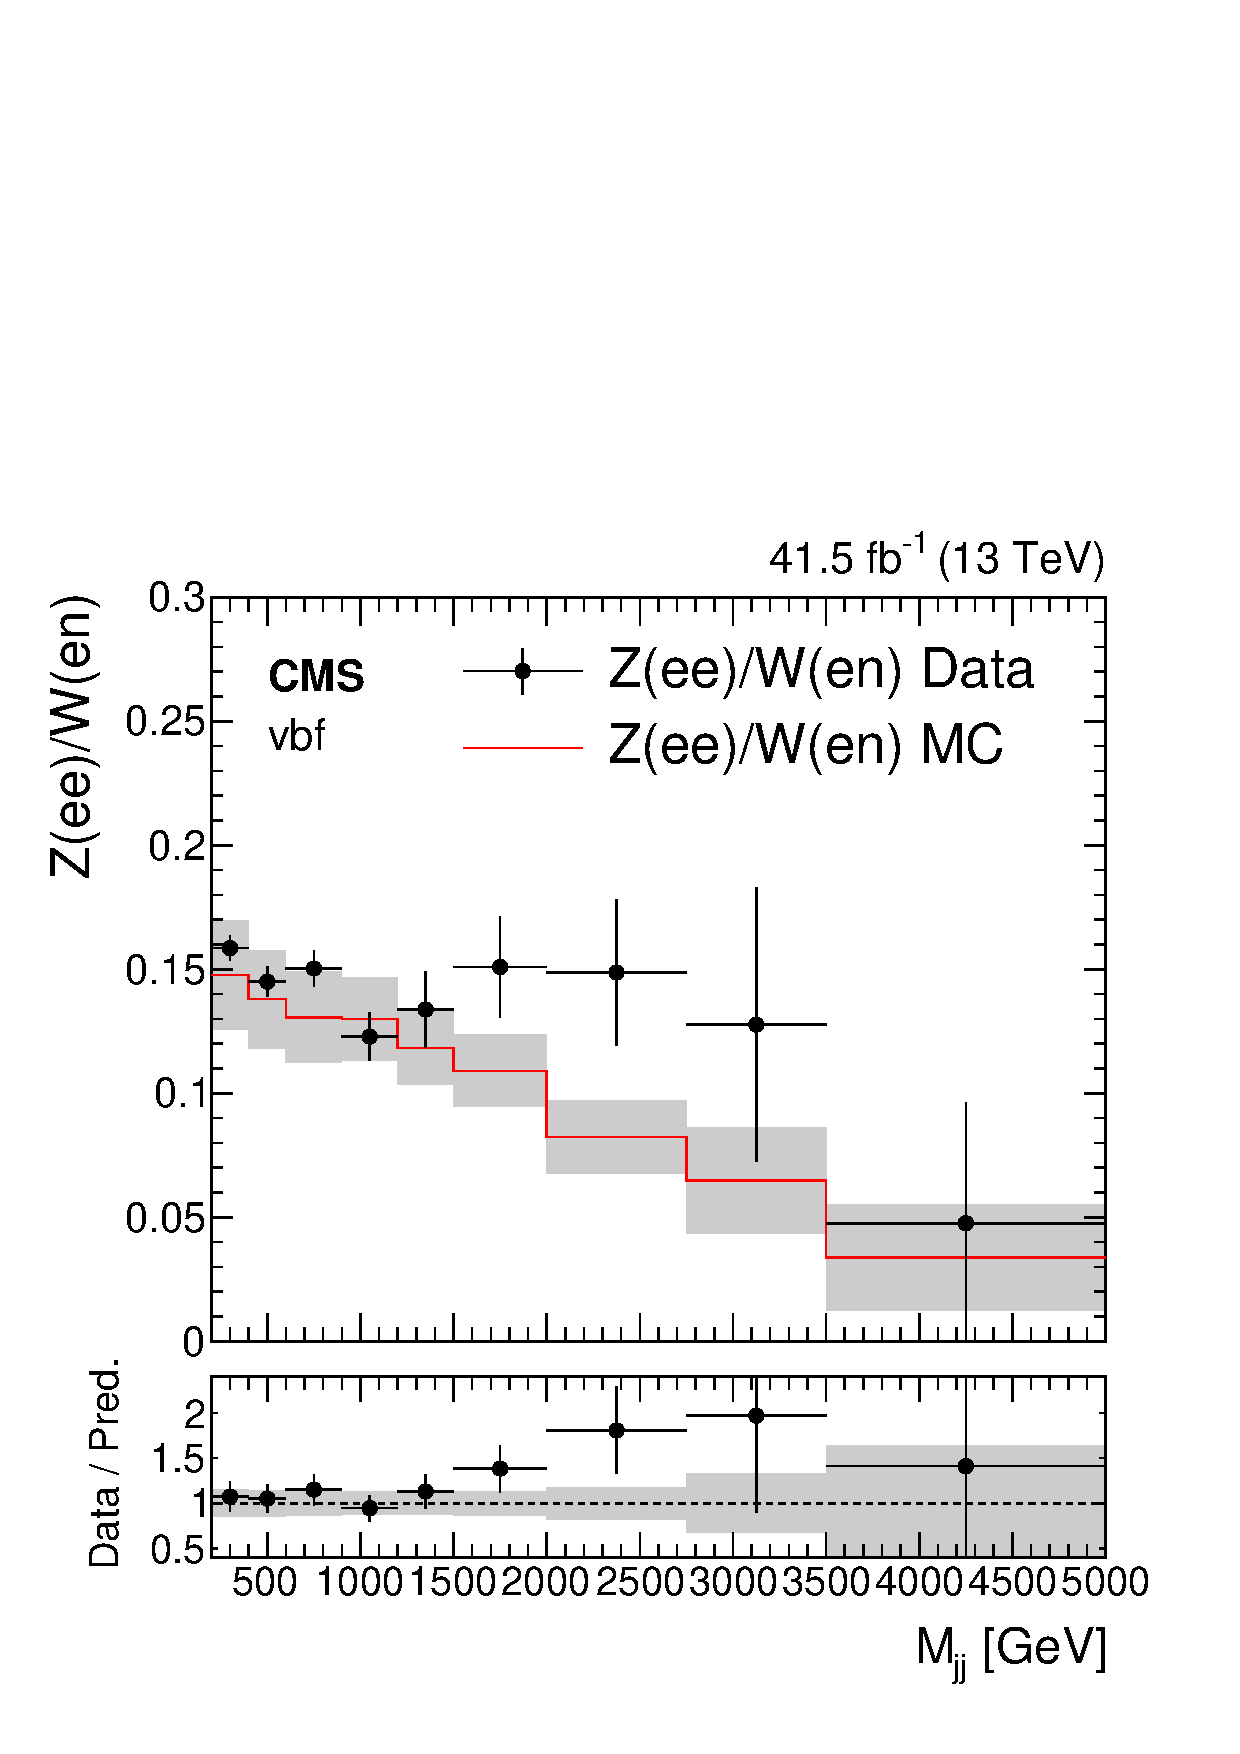
\includegraphics[width=0.45\textwidth]{\tfPlotDir/dielectron_singleelectron_cat_vbf_2017_2017ratio.pdf}
    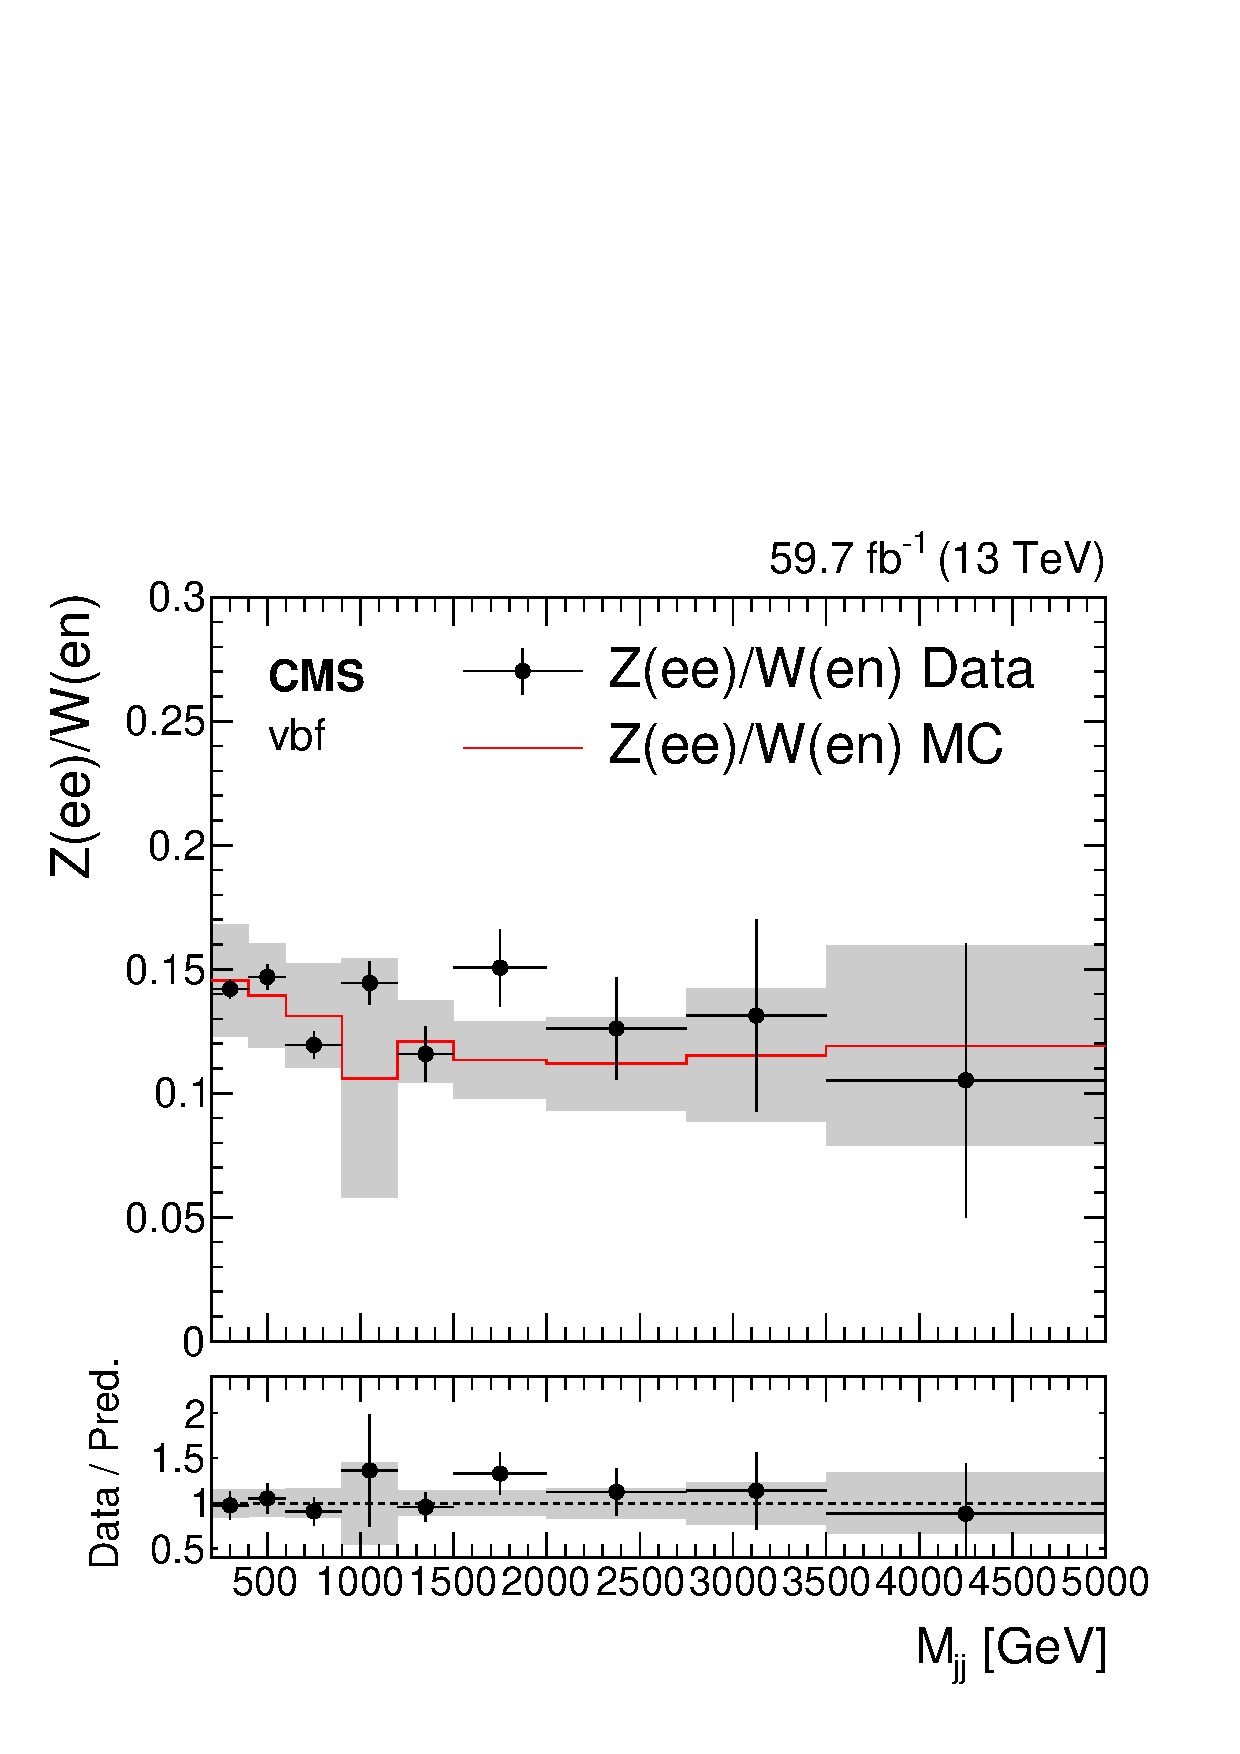
\includegraphics[width=0.45\textwidth]{\tfPlotDir/dielectron_singleelectron_cat_vbf_2018_2018ratio.pdf} \\
    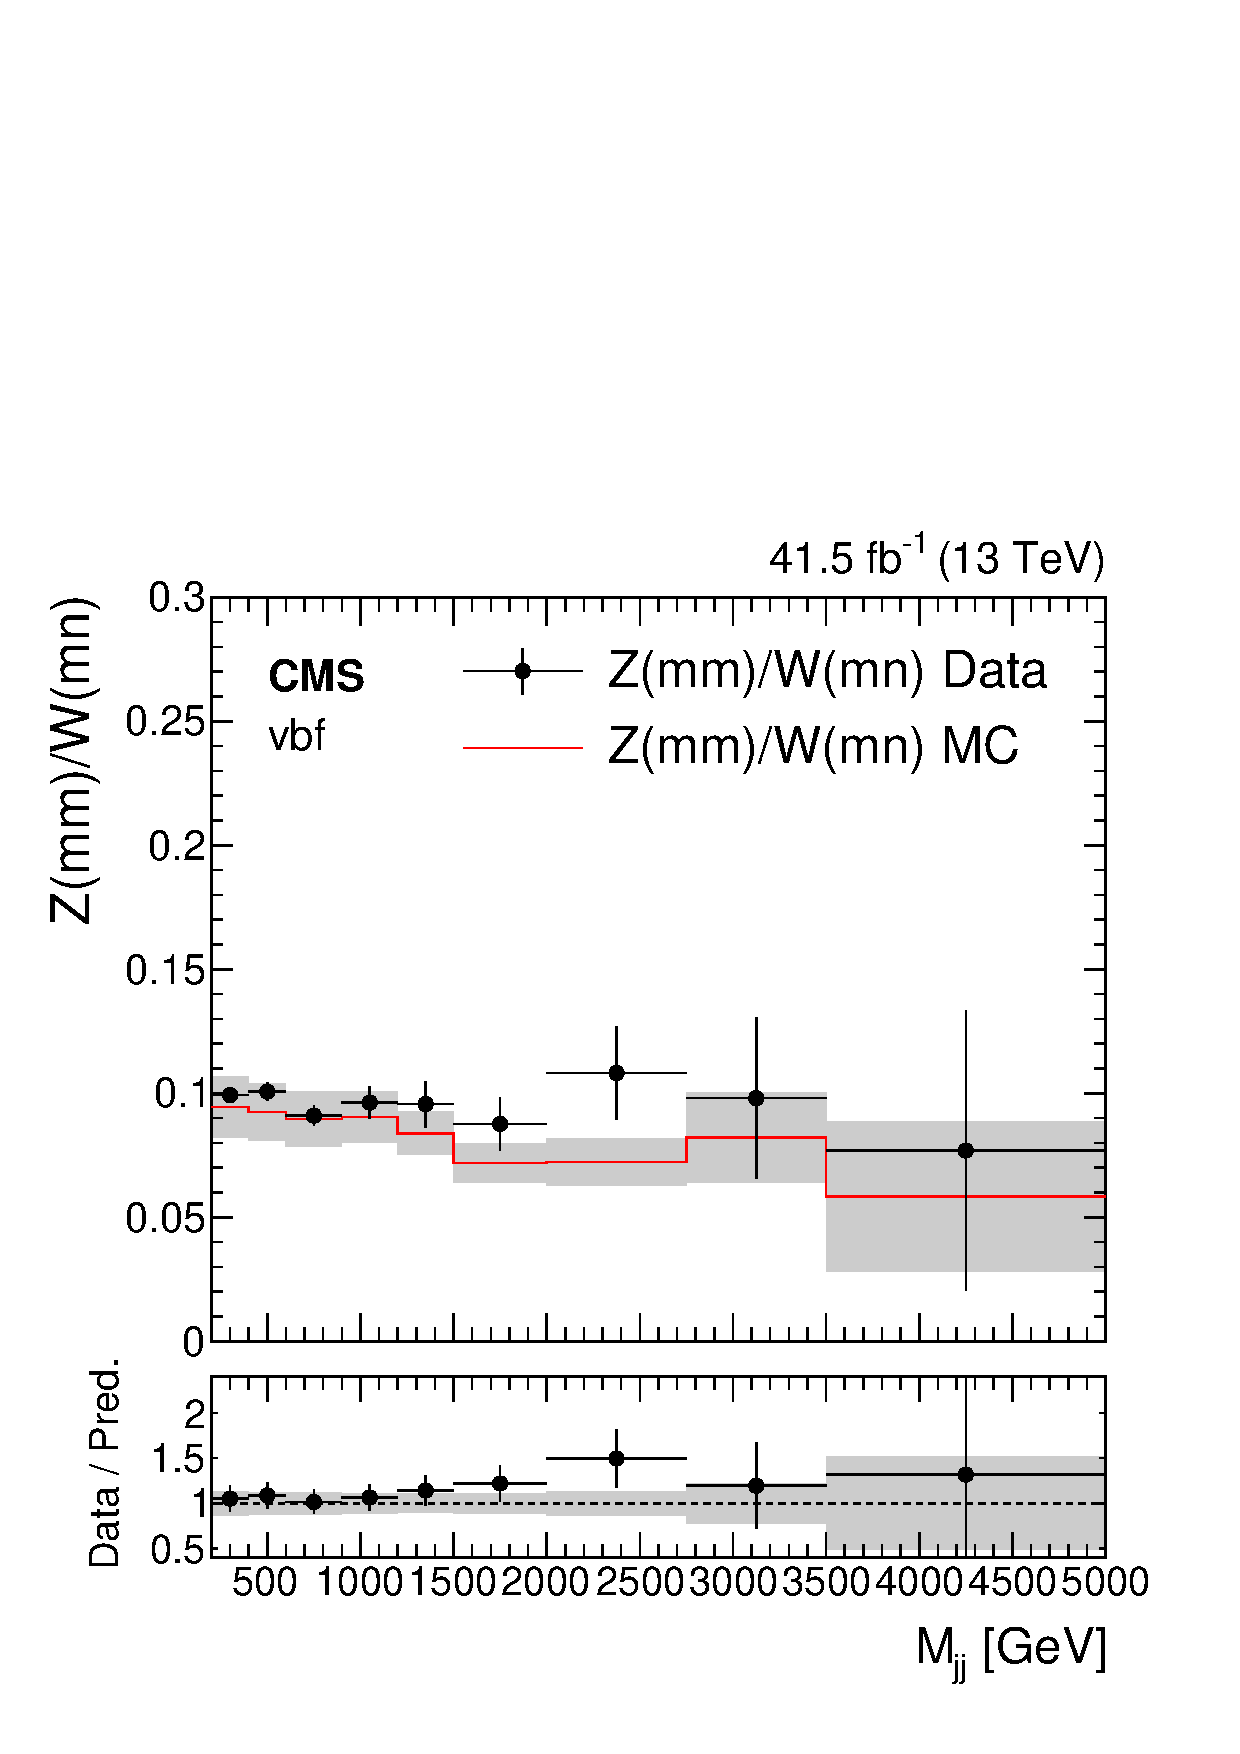
\includegraphics[width=0.45\textwidth]{\tfPlotDir/dimuon_singlemuon_cat_vbf_2017_2017ratio.pdf}
    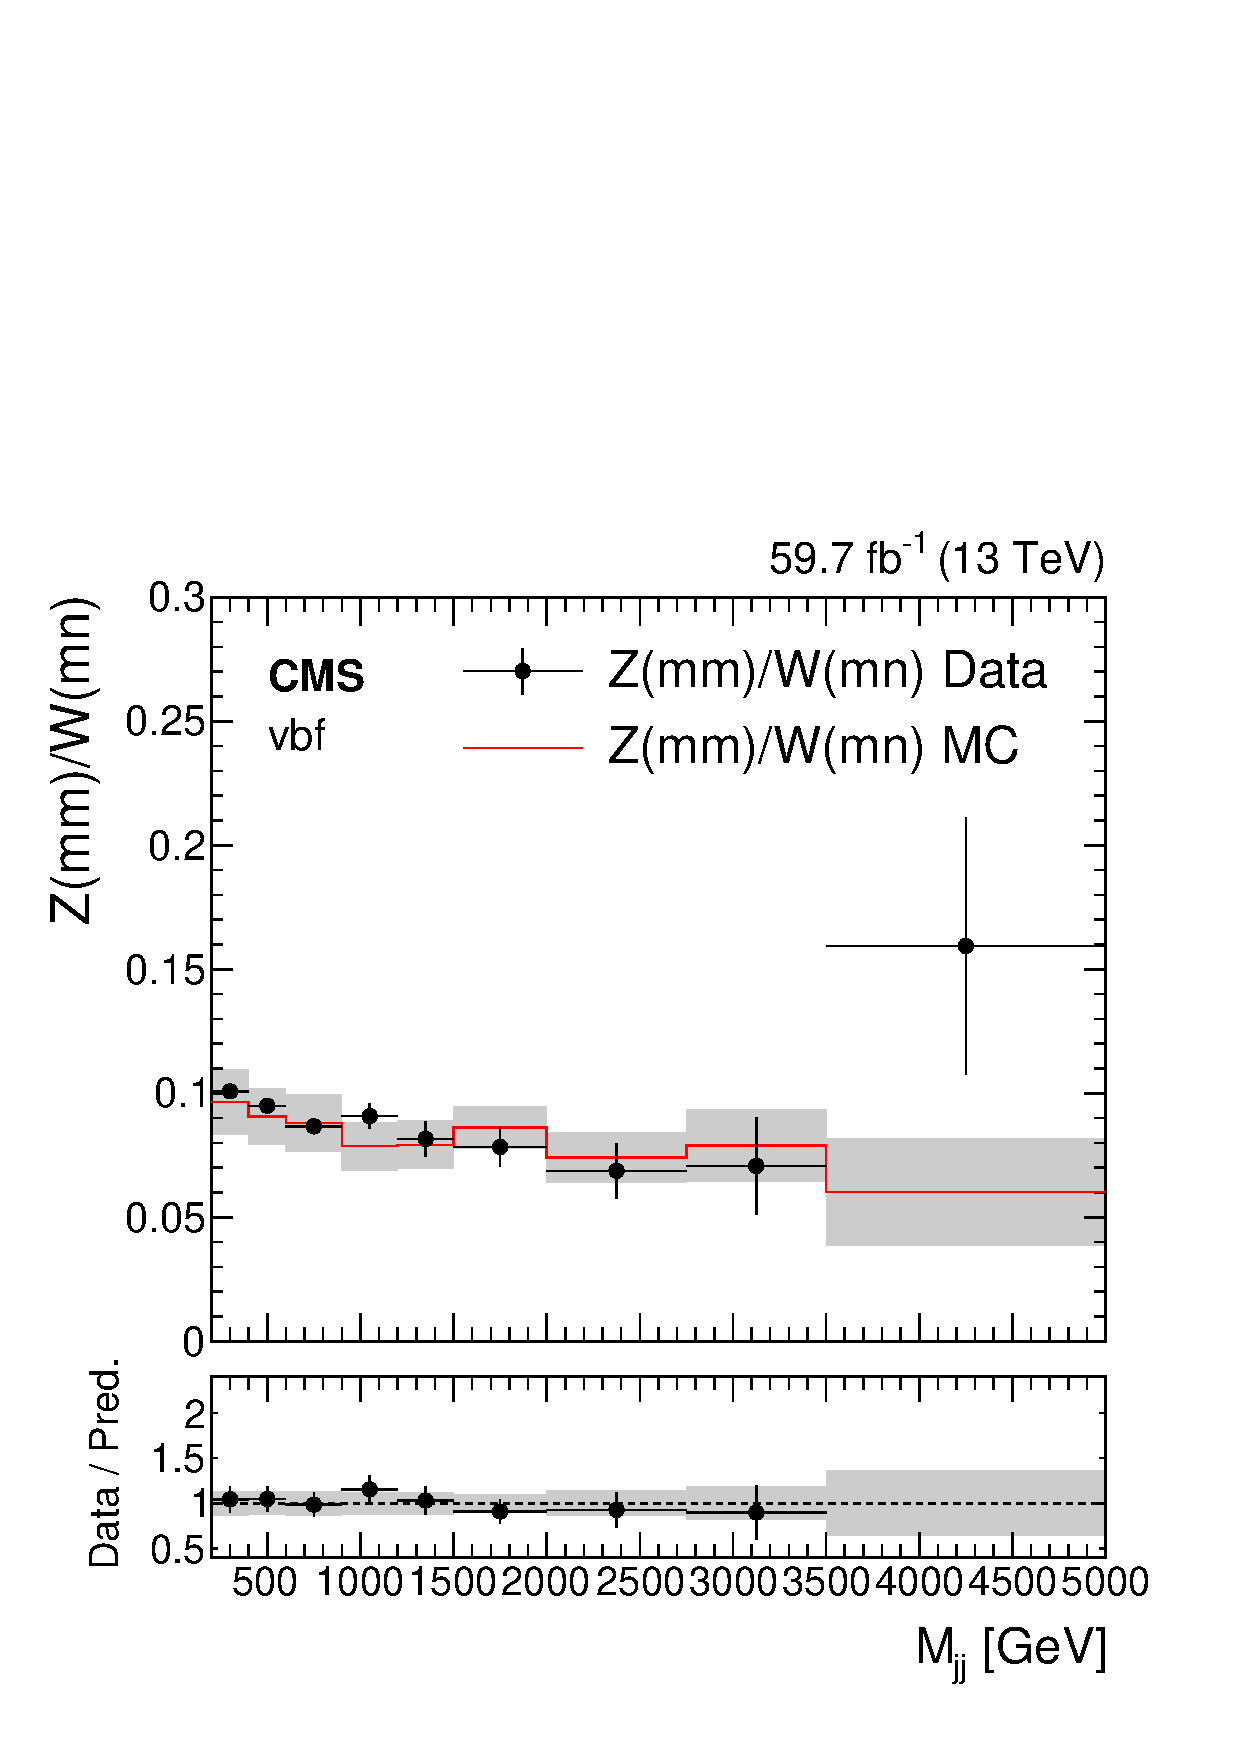
\includegraphics[width=0.45\textwidth]{\tfPlotDir/dimuon_singlemuon_cat_vbf_2018_2018ratio.pdf}
  \caption{Transfer factors between Z and W control regions as a function of the dijet 
    mass. Results for both 2017 (left) and 2018 (right) datasets are shown. Plots on the top row show the ratios
    between the electron regions, while the plots on the bottom show the ratios between muon regions. 
    The bands show the theoretical and experimental systematic uncertainties on the ratios.}
    \label{fig:transfer_factors_zoverw}
\end{figure}

To further constrain the $\Zvvjets$~background and to avoid statistical limitations, the $\Zvvjets$~process is also linked to the \phojets~process in the photon CR, 
using the same transfer factor scheme as for the control regions with two charged leptons. The transfer factor accounts for all differences in 
triggering and identification between these two regions. Those transfer factors are shown in Fig.~\ref{fig:transfer_factors_gamma}.

\begin{figure}[htbp]
    \centering
          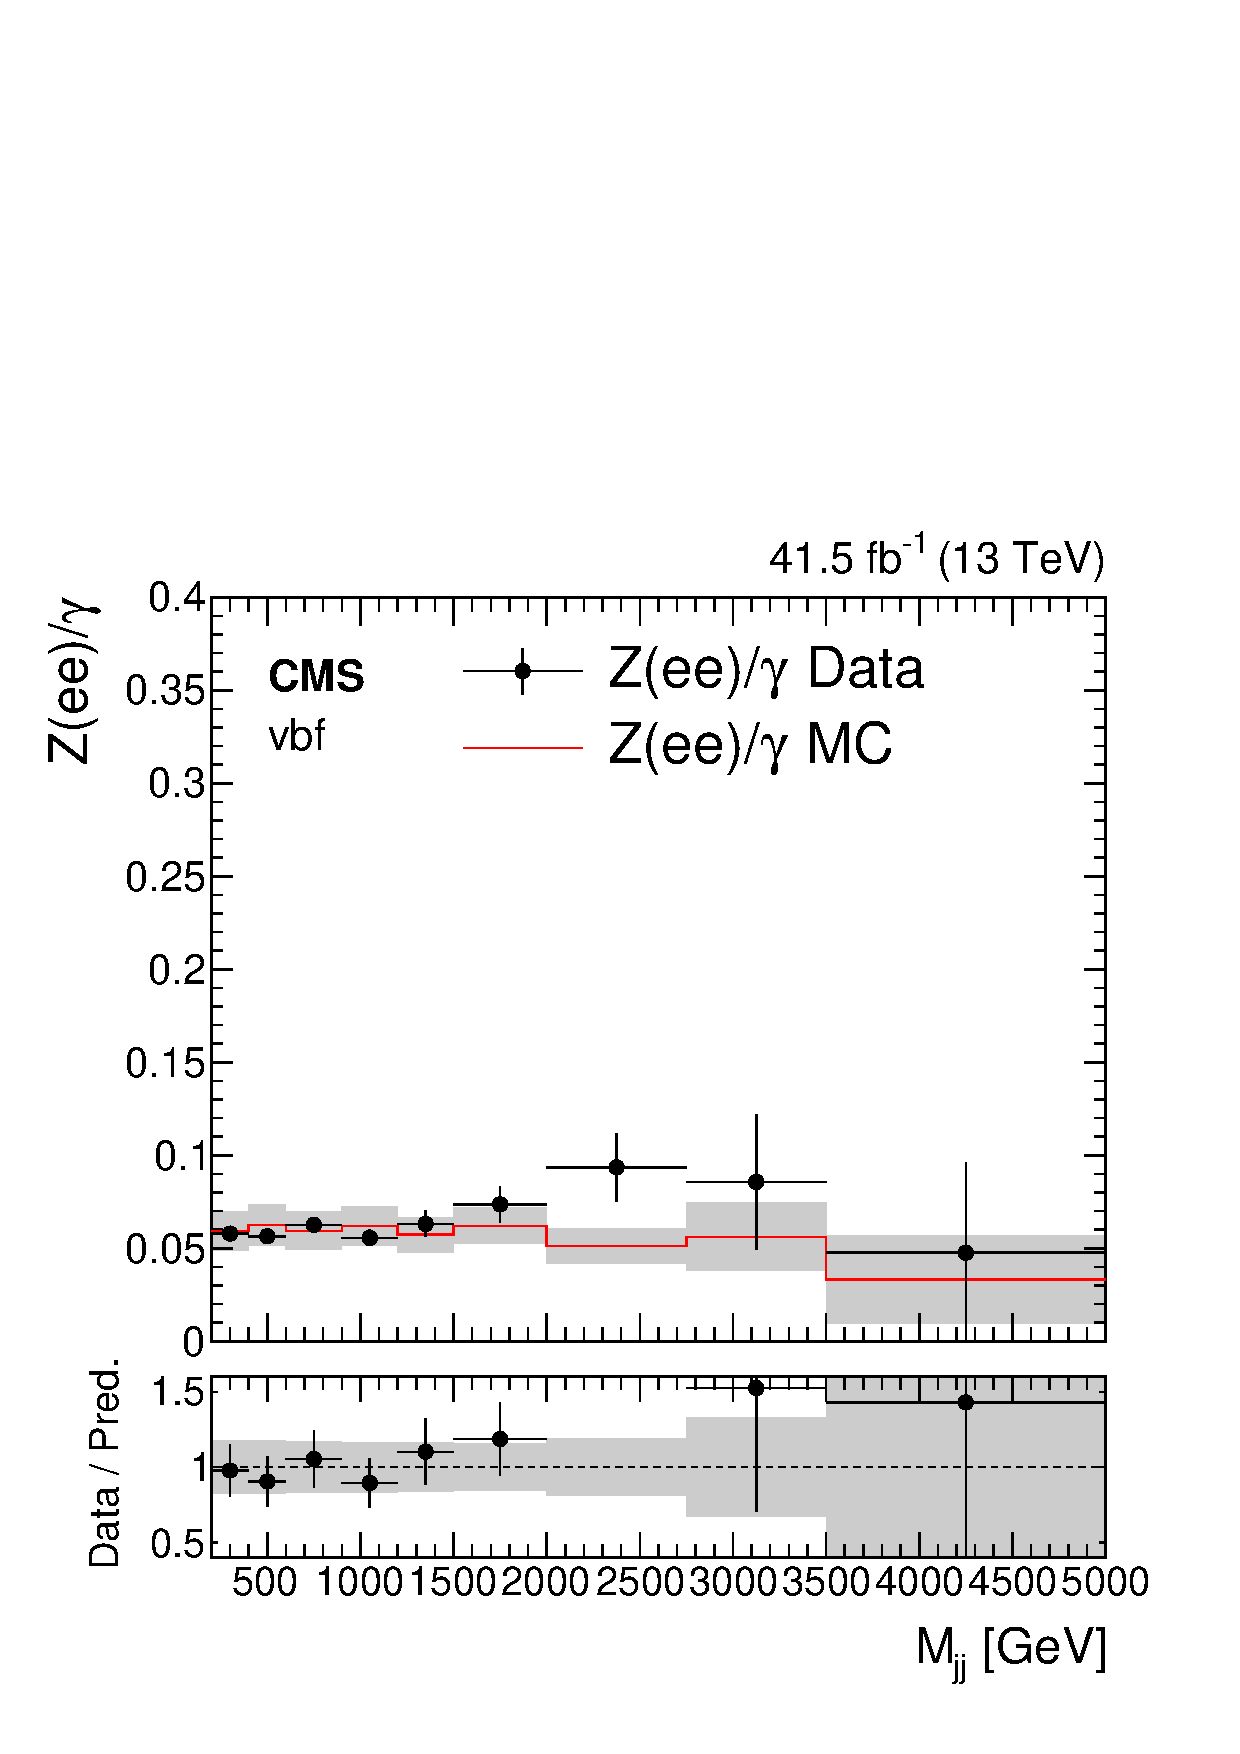
\includegraphics[width=0.45\textwidth]{\tfPlotDir/dielectron_gjets_cat_vbf_2017_2017ratio.pdf}
          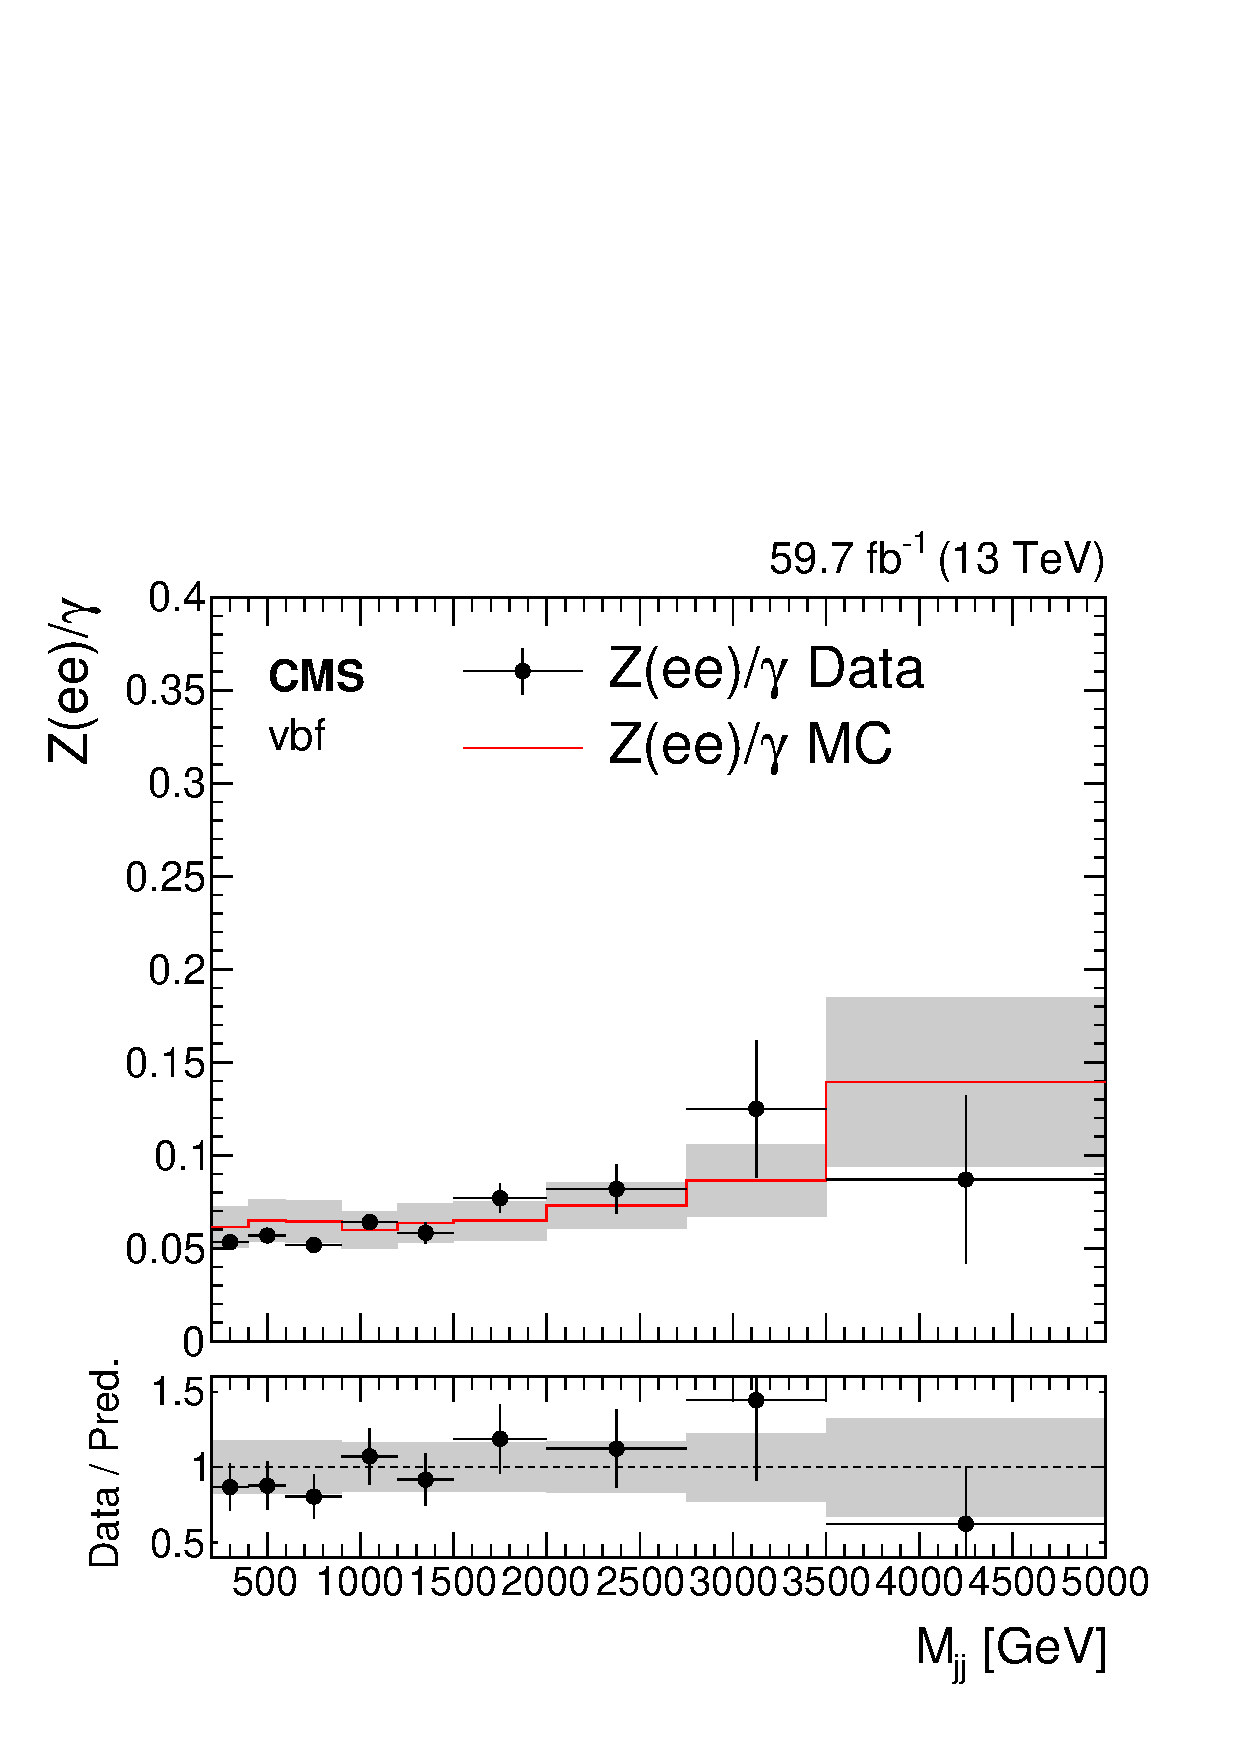
\includegraphics[width=0.45\textwidth]{\tfPlotDir/dielectron_gjets_cat_vbf_2018_2018ratio.pdf} \\
          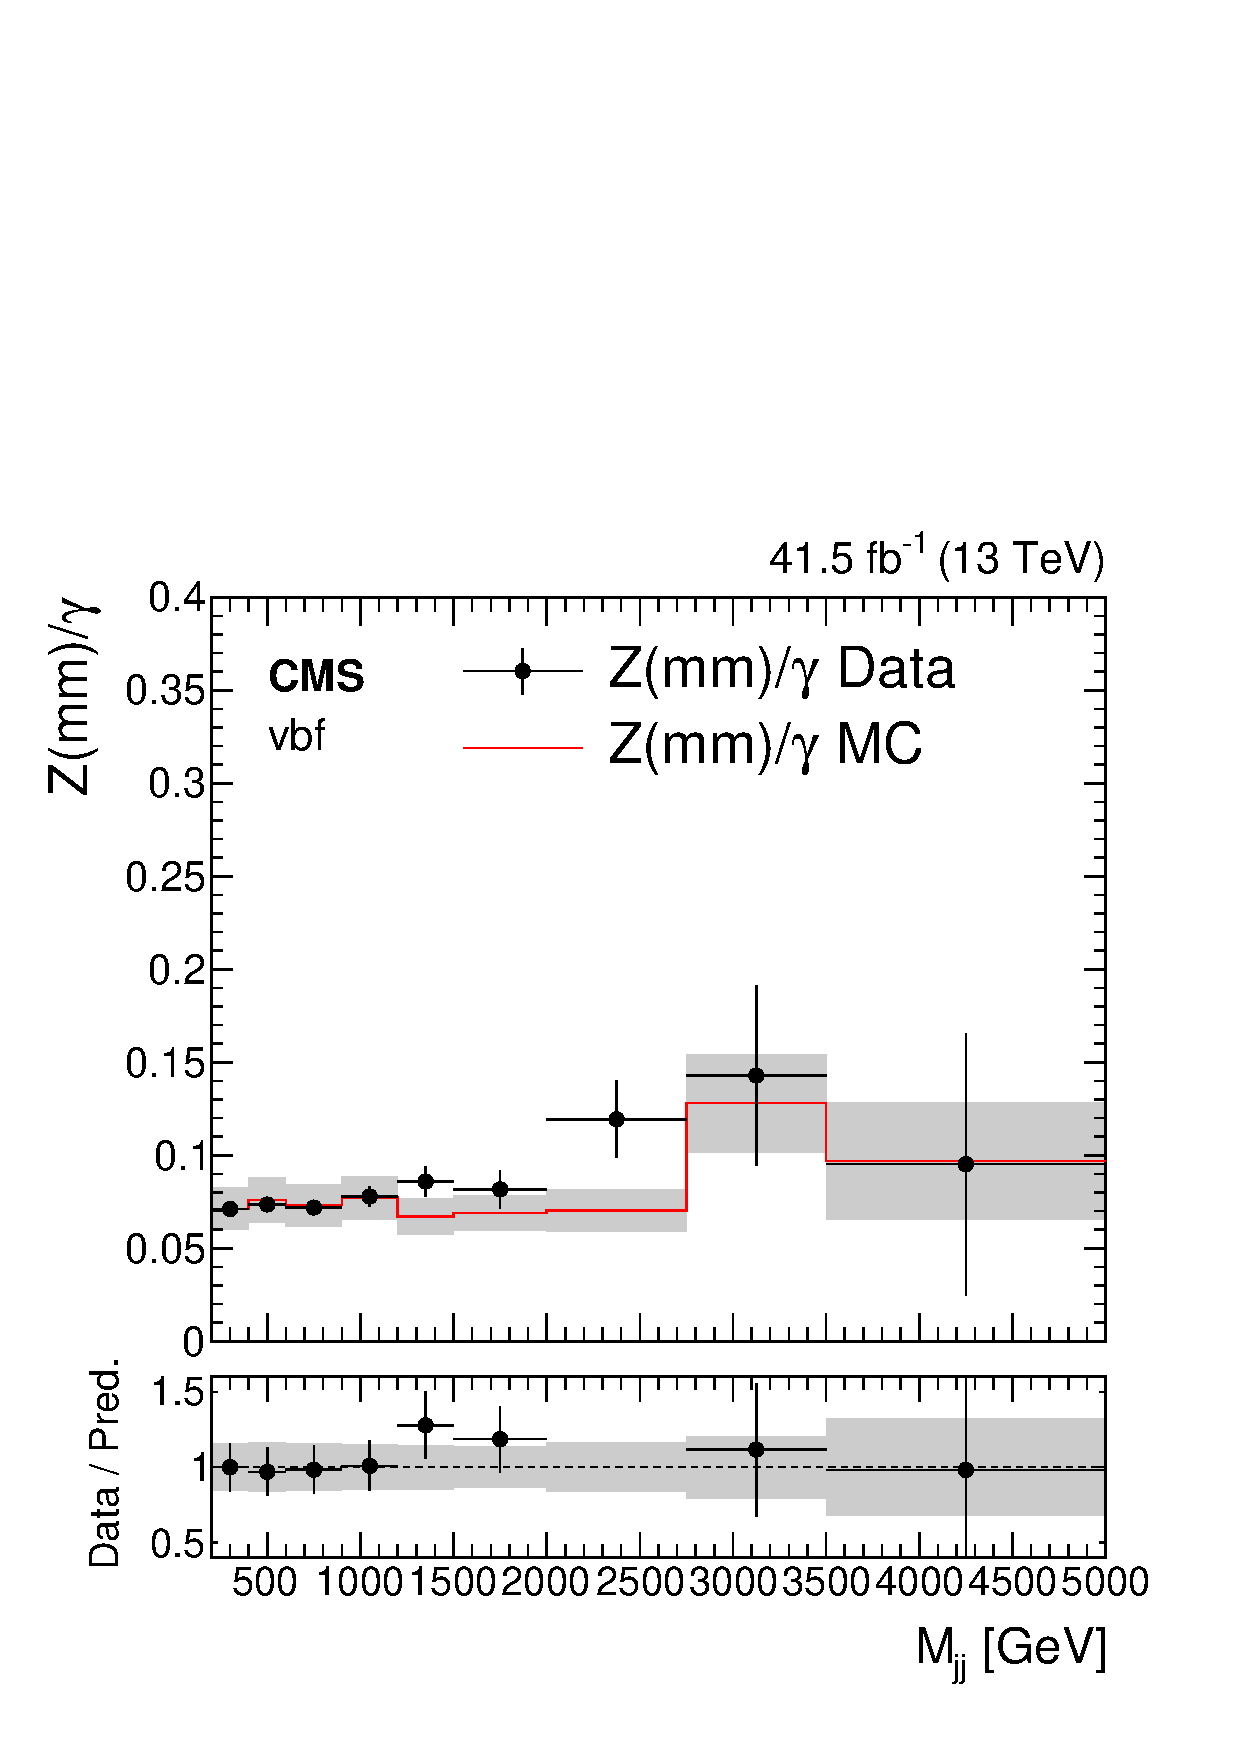
\includegraphics[width=0.45\textwidth]{\tfPlotDir/dimuon_gjets_cat_vbf_2017_2017ratio.pdf}
          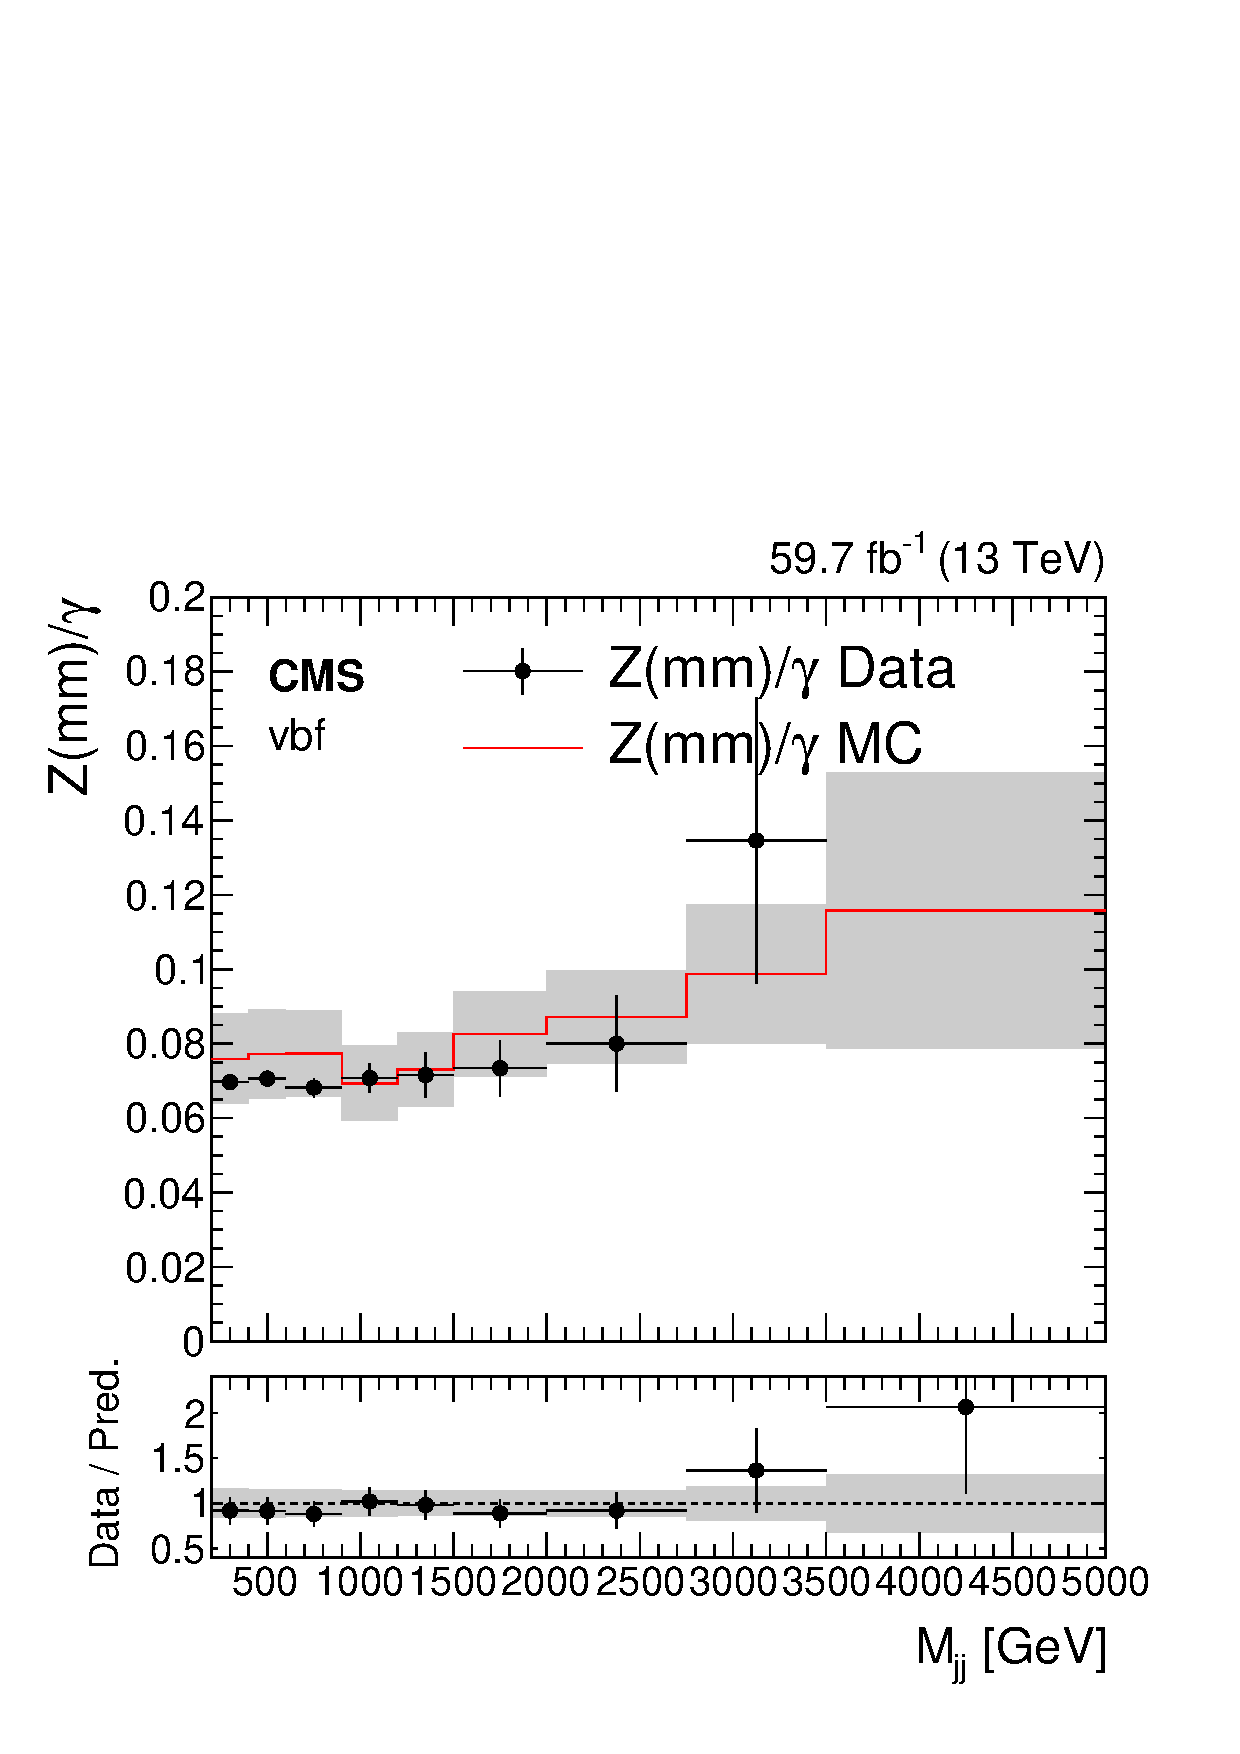
\includegraphics[width=0.45\textwidth]{\tfPlotDir/dimuon_gjets_cat_vbf_2018_2018ratio.pdf}
    \caption{Transfer factors for $\mathrm{Z}(ee) / \gamma +$ jets (top) and $\mathrm{Z}(\mu\mu) / \gamma +$ jets (bottom) processes. 
    Results with 2017 datasets are shown on the left column, and 2018 results are shown on the right column.
    The bands show the experimental systematic uncertainties on the ratios.}
    \label{fig:transfer_factors_gamma}
\end{figure}

\clearpage

\subsection{Systematic uncertainties}
\label{subsec:sys_uncertainties}

Systematic uncertainties in the transfer factors are modeled as constrained nuisance parameters and include both
experimental uncertainties and theoretical uncertainties in $\Wjets$ to $\Zjets$ and $\gamma \ +$ jets 
to $\Zjets$ cross section ratios. Theoretical and experimental uncertainties considered in the analysis are discussed
in the following two subsections.

\subsubsection{Theoretical uncertainties}

Theoretical uncertainties in $\Wjets$, $\Zjets$ and $\gamma \ +$ jets processes include effects from QCD and EWK higher-order
corrections along with the parton distribution function (PDF) modeling uncertainty. One of the uncertainties considered comes from the
variations around the central renormalization and factorization scale choice. It is evaluated by taking the differences in the NLO cross
section two-dimensionally as a function of boson \pt and \mjj~after changing the renormalization and factorization scales by a factor of two 
and a factor of one-half with respect to the default value. These constant scale variations mainly affect the
overall normalization of the boson \pt distributions. 
Uncertainty due to the parton distribution functions (PDF) on the k-factors
is evaluated using the recommendation from the PDF4LHC authors~\cite{paper:PDF4LHC}. 
This is added in quadrature with uncertainty due to the choice of $\alpha_{s}$, the coupling constant for the QCD interaction.
For the photon transfer factor, the procedure is identical with the exception that the uncertainties are estimated one-dimensionally versus boson \pt{}.

The scale uncertainties are treated as partially correlated between the \Zjets~and \Wjets~processes in the following fashion. 
For a certain scale uncertainty component (\textit{e.g.,} the factorization scale) the W$/$Z ratio is evaluated from the \Zjets{} and \Wjets~processes 
separately and the difference to the nominal value is calculated.
An envelope of the largest uncertainty out of the two processes is taken as the uncertainty on the ratio.
This is done for all of the theoretical uncertainty components on the ratios.
It is observed that the contribution from varying the \Wjets~process is the larger uncertainty source,
hence taking the envelope equates to taking the \Wjets~uncertainty contribution only and ignoring that from the Z.

The PDF uncertainties are treated as fully correlated between the \Zjets~and \Wjets~processes. For up and down variations of the PDF, W$/$Z ratio is 
evaluated by varying the \Wjets~and \Zjets~processes simultaneously, and the varied W$/$Z ratio is calculated accordingly. 
Both for the scale and PDF uncertainties, a similar correlation scheme is applied while computing the uncertainties for $\gamma~/~\Zjets$ ratio.

The full set of theory uncertainties on the W$/$Z and $\gamma/$Z ratios are shown in Fig.~\ref{fig:theory_uncs}. On the top row,
the uncertainties for QCD W$/$Z ratio (left) and VBF W$/$Z ratio (right) are shown. On the bottom row,
the uncertainties for QCD $\gamma/$Z ratio (left) and VBF $\gamma/$Z ratio (right) are shown. All uncertainties are shown as a function
of the dijet invariant mass, $\mjj$. 

\begin{figure}[htbp]
  \centering
    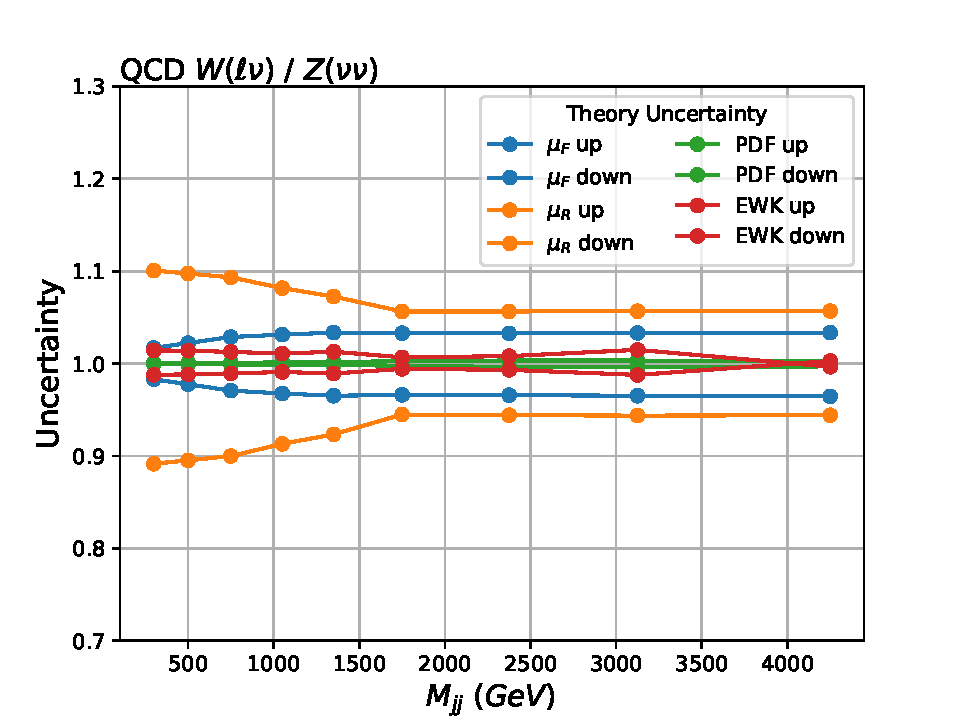
\includegraphics[width=0.45\textwidth]{TheoryUncertainties/uncertainty_ratio_z_qcd_mjj_unc_zoverw_nlo_2018.pdf}
    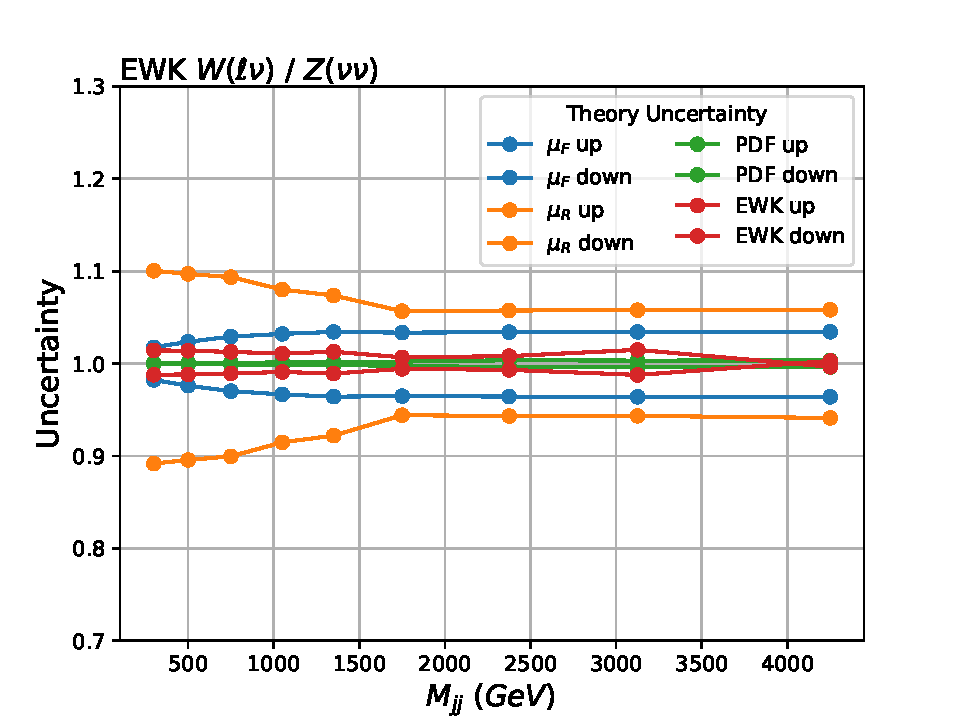
\includegraphics[width=0.45\textwidth]{TheoryUncertainties/uncertainty_ratio_z_ewk_mjj_unc_zoverw_nlo_2018.pdf} \\
    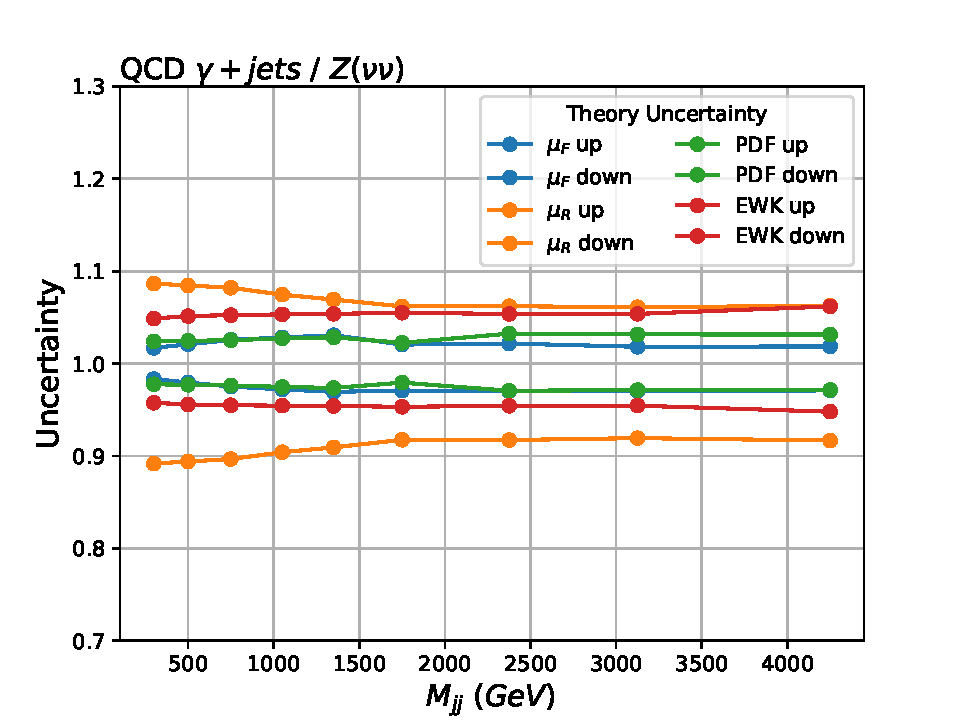
\includegraphics[width=0.45\textwidth]{TheoryUncertainties/uncertainty_ratio_gjets_qcd_mjj_unc_goverz_nlo_2018.pdf}
    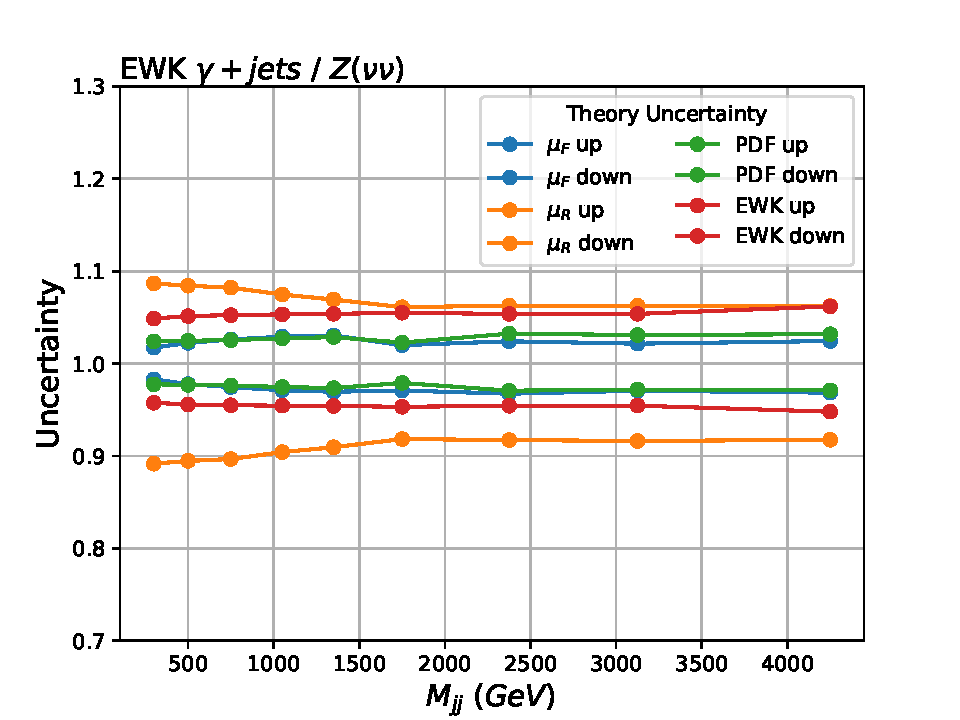
\includegraphics[width=0.45\textwidth]{TheoryUncertainties/uncertainty_ratio_gjets_ewk_mjj_unc_goverz_nlo_2018.pdf}
  \caption{Theoretical uncertainties on W$/$Z (top) and $\gamma/$Z (bottom) transfer factors. Uncertainties are calculated as a
  function of $\mjj$. Uncertainties for QCD ratios are shown on the left column, while uncertainties for EWK ratios are shown on the right column.}
  \label{fig:theory_uncs}
\end{figure}

From Fig.~\ref{fig:theory_uncs}, it can be observed that the dominating theory uncertainty, is the renormalization
scale uncertainty, which reaches to around $10\%$ at lower $\mjj$. It can also be observed that the PDF uncertainties are typically smaller compared to
other theoretical uncertainty sources. This is mainly due to them being fully correlated between different $\Vjets$ processes, resulting in large cancellations 
in the ratios. 

\clearpage

\subsubsection{Experimental uncertainties}

Experimental uncertainties include uncertainties on the lepton reconstruction and identification criteria, jet energy scale and resolution, 
pileup reweighting, and prefire reweighting.

Uncertainties on veto weights are applied for electrons, muons, taus and b jets. For the case of electrons and muons, the uncertainties are split
into identification and isolation uncertainties, in accordance with the weight definitions for these objects, as defined in Sec.~\ref{subsec:lepton_id_reweighting}.
These uncertainties are typically not correlated with the kinematics of the two VBF jets, and hence $\mjj$. Therefore, no significant shape as a function of $\mjj$ 
is observed for these uncertainties, and flat uncertainties are applied. These uncertainties are summarized in Table.~\ref{tab:systematics}.

The uncertainty on the prefire reweighting, as explained in Sec.~\ref{subsec:prefiring_weighting}, is computed by varying the prefire weight
within its uncertainties, and computing the impact on the $\mjj$ distribution. The variations in the $\mjj$ shape are computed from the VBF $\hinv$
signal sample, and the resulting shapes are applied to all $\hinv$ samples as a shape uncertainty. For minor backgrounds,
a $3\%$ flat uncertainty is applied instead, which is observed to be a good approximation of the uncertainty. Since prefire reweighting is done only
on 2017 data, this uncertainty is only applied to 2017 data.
The uncertainty on the prefiring weights as a function of $\mjj$ is shown in Fig.~\ref{fig:l1prefire_unc}.
Similar to the prefire reweighting uncertainty, the uncertainty on pileup reweighting (explained in Sec.~\ref{subsec:pu_reweighting}) is done by varying the pileup
weight within its uncertainties, and computing the impact on the $\mjj$ distribution per process. The uncretainty due to the pileup reweighting is found to be $O(1\%)$.

\begin{figure}[htbp]
  \centering
  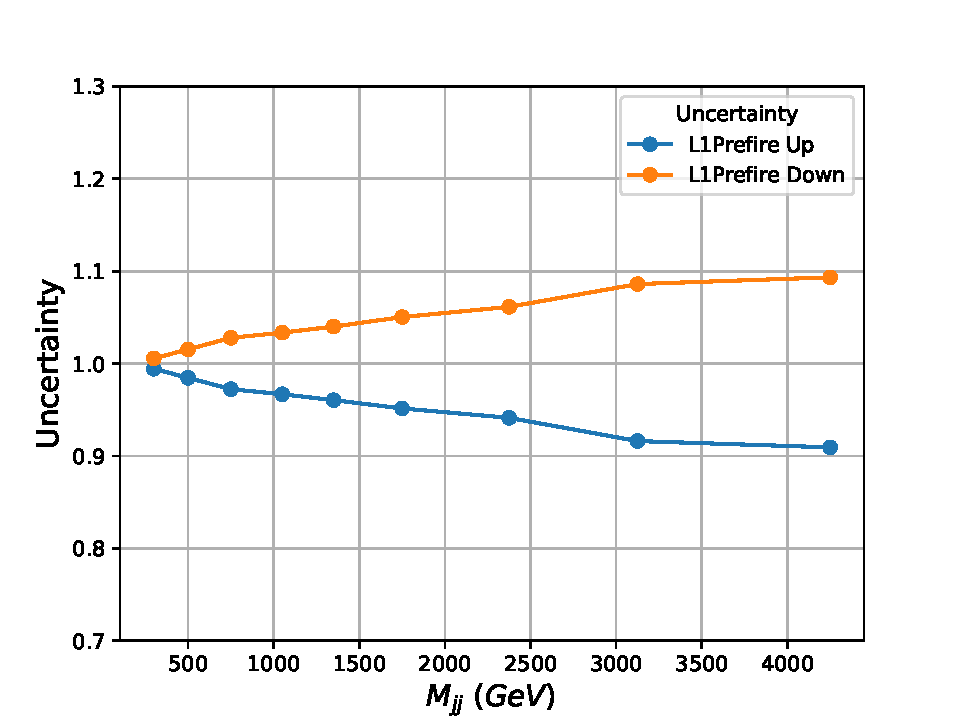
\includegraphics[width=0.7\textwidth]{ExperimentalUncertainties/L1prefire_unc.pdf}
  \caption{Uncertainty due to the L1 prefire reweighting as a function of $\mjj$. The uncertainty is computed from VBF $\hinv$
  signal sample by varying the prefiring weight within its uncertainty. This uncertainty is applied as a shape uncertainty to all
  $\hinv$ signals considered in the analysis.}
  \label{fig:l1prefire_unc}
\end{figure}

% , and the computed shape variations in $\mjj$ are applied as shape uncertainties in the analysis. This uncertainty is shown in Fig.~\ref{fig:pu_uncs_vbfh}.

% \begin{figure}[htbp]
%   \centering
%   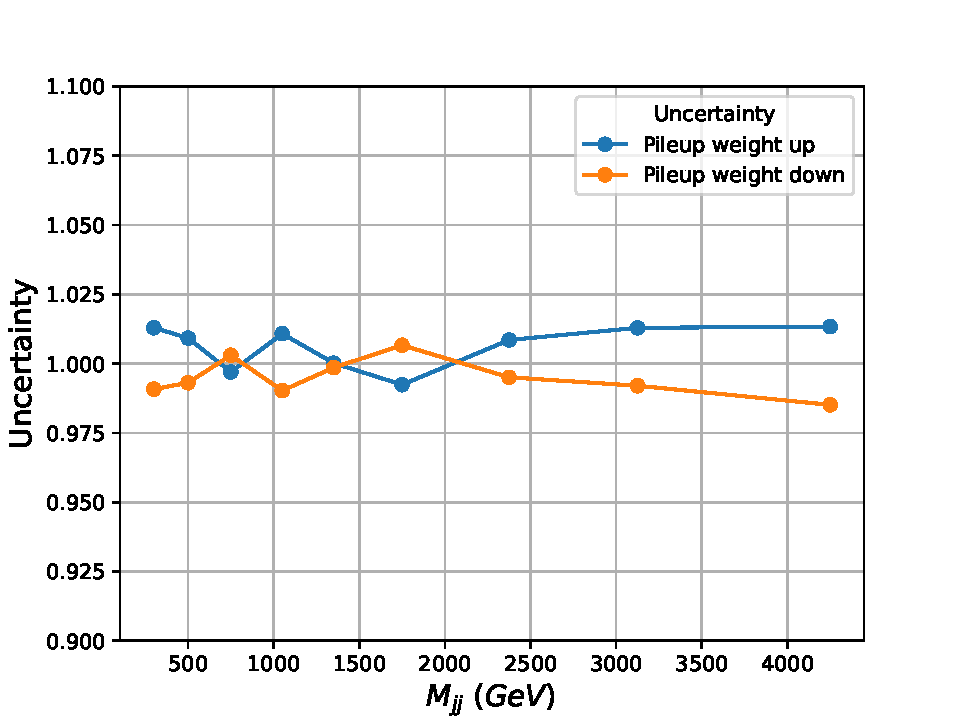
\includegraphics[width=0.7\textwidth]{ExperimentalUncertainties/VBFH_pileup_unc.pdf}
%   \caption{Uncertainty due to pileup reweighting as a function of $\mjj$. The uncertainty is computed from VBF $\hinv$
%   signal sample by varying the pileup weight within its uncertainty.}
%   \label{fig:pu_uncs_vbfh}
% \end{figure}

The uncertainty in the modeling of $\ptmiss$ in simulation~\cite{Khachatryan:2014gga} is dominated by the uncertainty on the jet energy scale (JES) 
and resolution (JER). The effect is estimated by varying the $\pt$ of VBF jets within their uncertainty, propagating the effect to $\ptmiss$, and then 
performing the full analysis selection based on the varied inputs. For JES uncertainties, this variation is done for 11 sub sources, where each 
sub-source is defined in accordance with the correlation scheme defined by JetMET POG, which can be found in \cite{jetMET_twiki}. The uncertainties for JES and
JER are applied both to the transfer factors, and to the individual processes such as signal processes and minor backgrounds.

In the transfer factors, the majority of the JES and JER uncertainties cancel, but residual non-cancellation is observed. The residual uncertainty 
remaining in the ratios is found to be approximately $2\%$. For the transfer factors, a flat single-bin uncertainty is assigned for each
JES and JER uncertainty source for each ratio. All the JES and JER uncertainties for 
the Z(SR)/Z(CR) ($\Zmmjets$ and $\Zeejets$ channels combined for Z(CR)) ratio are shown in Fig.~\ref{fig:znunu_over_zll_jes_jer_uncs}. 
The uncertainties for Z(SR)/$\gamma$ are shown in Fig~\ref{fig:znunu_over_gjets_jes_jer_uncs}. 
% Generally, the uncertainties are smaller for the 2018 dataset, especially the uncertainty in the JER.

\begin{figure}[h!]
  \centering
  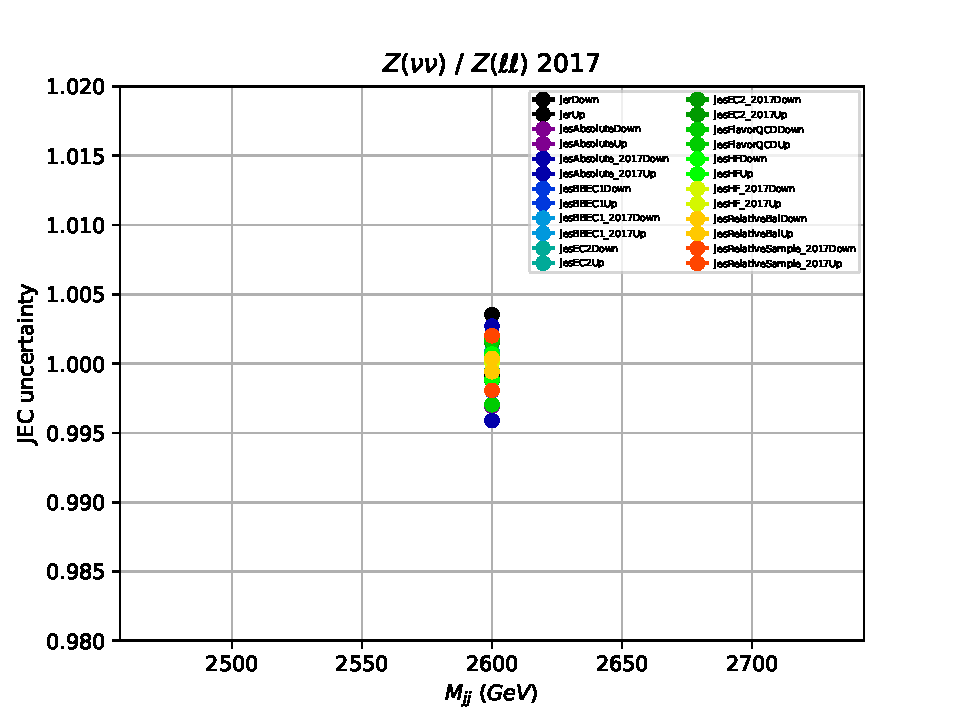
\includegraphics[width=0.49\textwidth]{ExperimentalUncertainties/JEC/znunu_over_zll17_qcd_splitJEC_singleBin.pdf}
  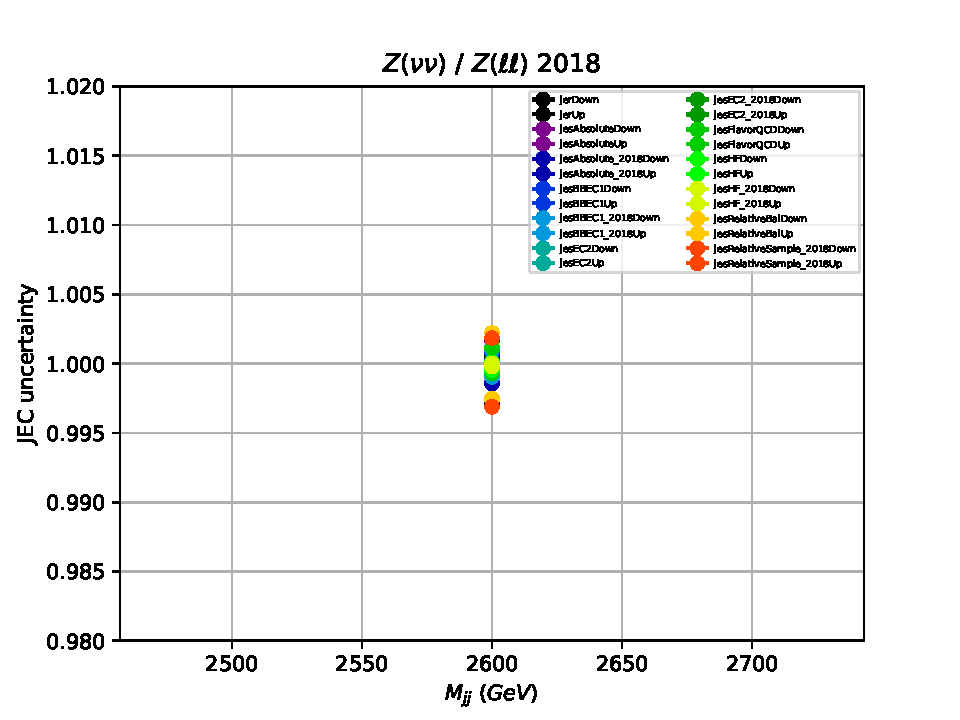
\includegraphics[width=0.49\textwidth]{ExperimentalUncertainties/JEC/znunu_over_zll18_qcd_splitJEC_singleBin.pdf}
  \caption{All single-bin JES/JER uncertainties on QCD Z(SR)/Z(CR) ratio for 2017 (left) and 2018 (right). 
    The black dot shows the JER uncertainty, and the others show up and down variation from all 11 JES sub sources. 
    All jet energy scale and resolution uncertainties cancel to within less than $1\%$.
  }
  \label{fig:znunu_over_zll_jes_jer_uncs}
\end{figure}

\begin{figure}[h!]
  \centering
  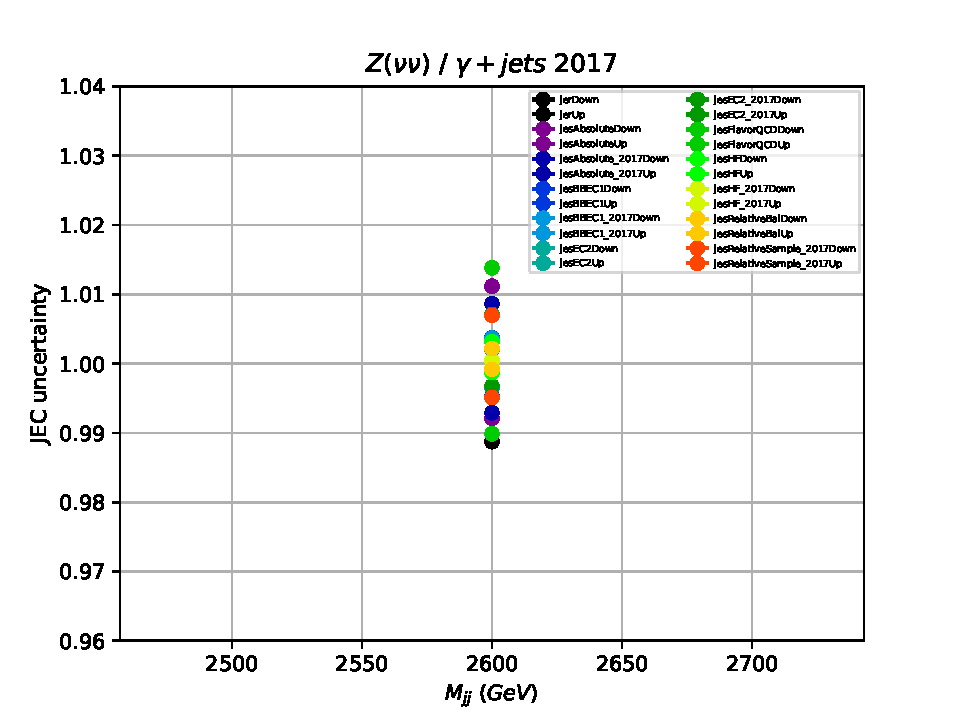
\includegraphics[width=0.49\textwidth]{ExperimentalUncertainties/JEC/znunu_over_gjets17_qcd_splitJEC_singleBin.pdf}
  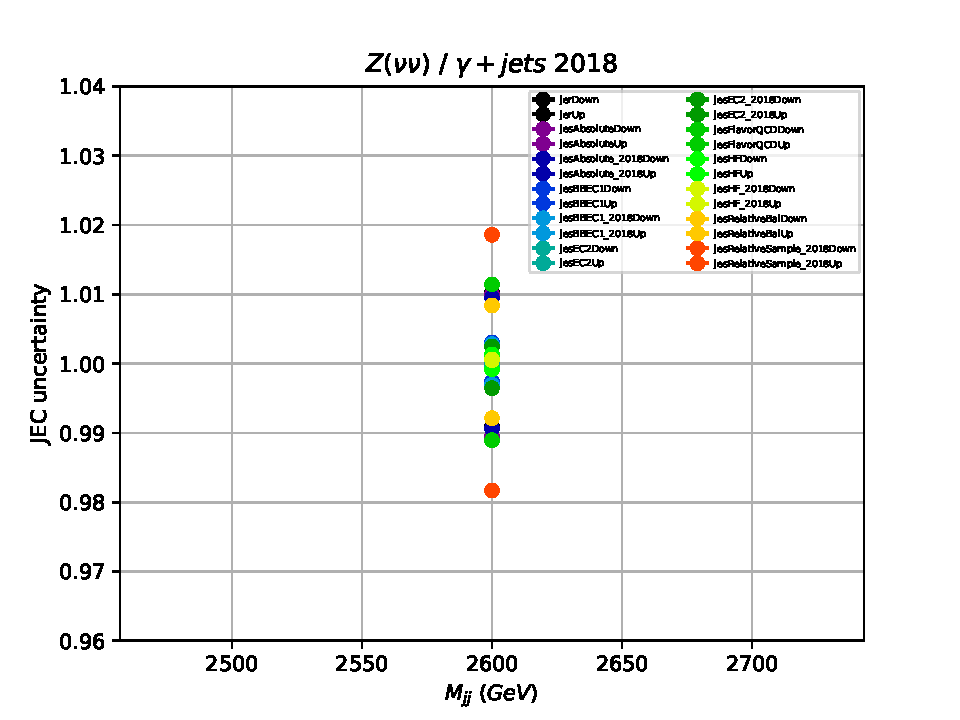
\includegraphics[width=0.49\textwidth]{ExperimentalUncertainties/JEC/znunu_over_gjets18_qcd_splitJEC_singleBin.pdf}
  \caption{All single-bin JES/JER uncertainties on QCD Z(SR)/$\gamma$ ratio for 2017 (left) and 2018 (right). 
    The black dot shows the JER uncertainty, and the others show up and down variation from all 11 JES sub-sources. 
    All jet energy scale and resolution uncertainties cancel within up to $2\%$.
  }
  \label{fig:znunu_over_gjets_jes_jer_uncs}
\end{figure}

The JES and JER uncertainties on minor backgrounds and signals are calculated in a very similar way as for the transfer factors. 
For these, the uncertainties are derived as a function of $\mjj$ for each jet energy uncertainty source. The uncertainties for minor backgrounds (top, diboson)
are derived using the strong $\Zvvjets$ sample, due to the limited statistics from the minor backgrounds. The uncertainties for $\hinv$ signal samples 
are derived from VBF $\hinv$ sample.
Most jet energy uncertainty sources are found to be on the order of $1\%$, while the uncertainty coming from the relative corrections are typically
found to be the dominating ones, also displaying an increasing shape as a function of $\mjj$, reaching to $\mathcal{O}(10\%)$ uncertainty levels at high $\mjj$.

The most dominating uncertainty source is the ``Relative Sample'' uncertainty, which is the jet $\eta$-dependent uncertainty due to different
residual jet energy corrections obtained by measurement from different channels, such as dijet events, $\gamma+$ jet events and Z$+$ jet events.
For these larger uncertainty sources, a second-degree polynomial is fit to smooth out the uncertainty shape. For smaller jet energy uncertainty sources,
a line fit is performed instead. For most jet energy uncertainty sources, no significant shape is observed as a function of $\mjj$.
The dominating jet energy uncertainty source, ``Relative Sample", 
is plotted in Fig.~\ref{fig:znunu_jec_uncs} for QCD $\Zvvjets$ and VBF $\hinv$ samples.

\begin{figure}[h!]
  \centering
  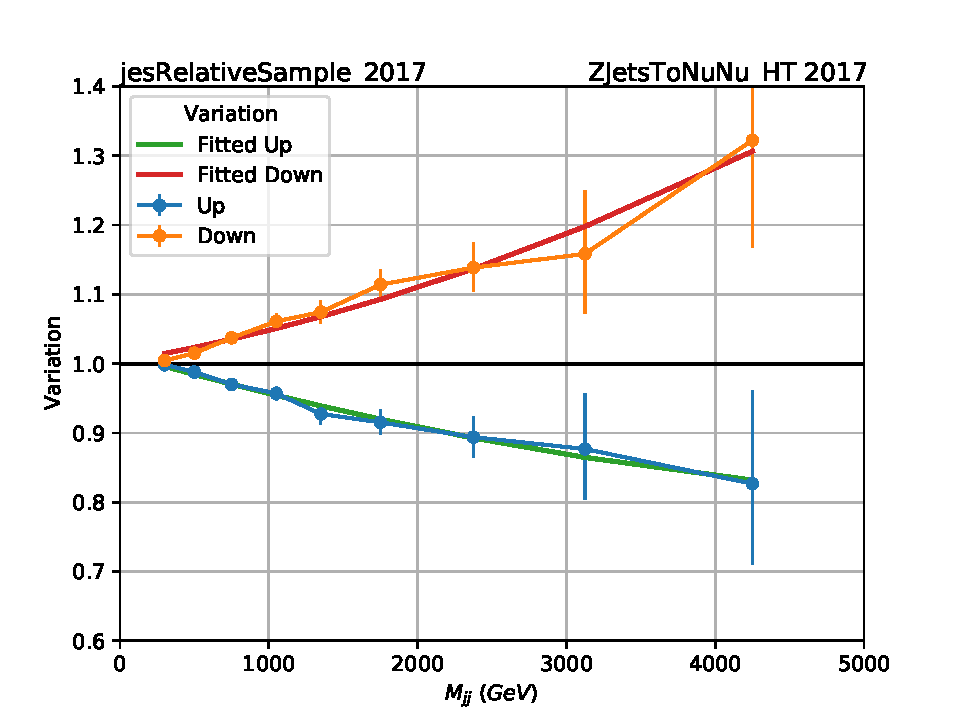
\includegraphics[width=0.49\textwidth]{ExperimentalUncertainties/JEC/ZJetsToNuNu_HT_2017_jesRelativeSample_2017.pdf}
  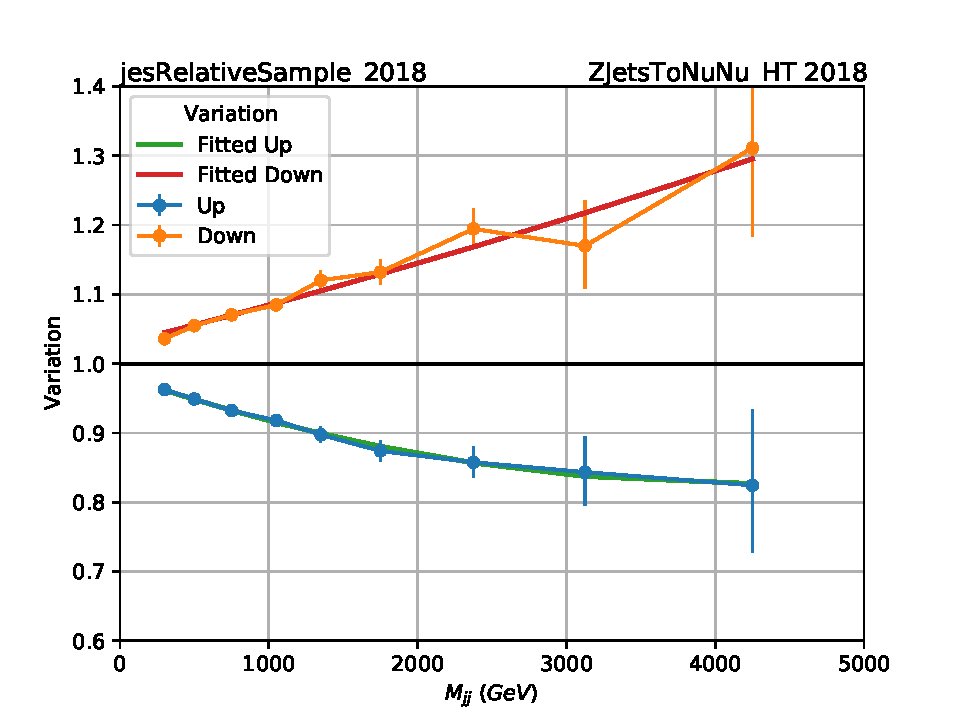
\includegraphics[width=0.49\textwidth]{ExperimentalUncertainties/JEC/ZJetsToNuNu_HT_2018_jesRelativeSample_2018.pdf} \\
  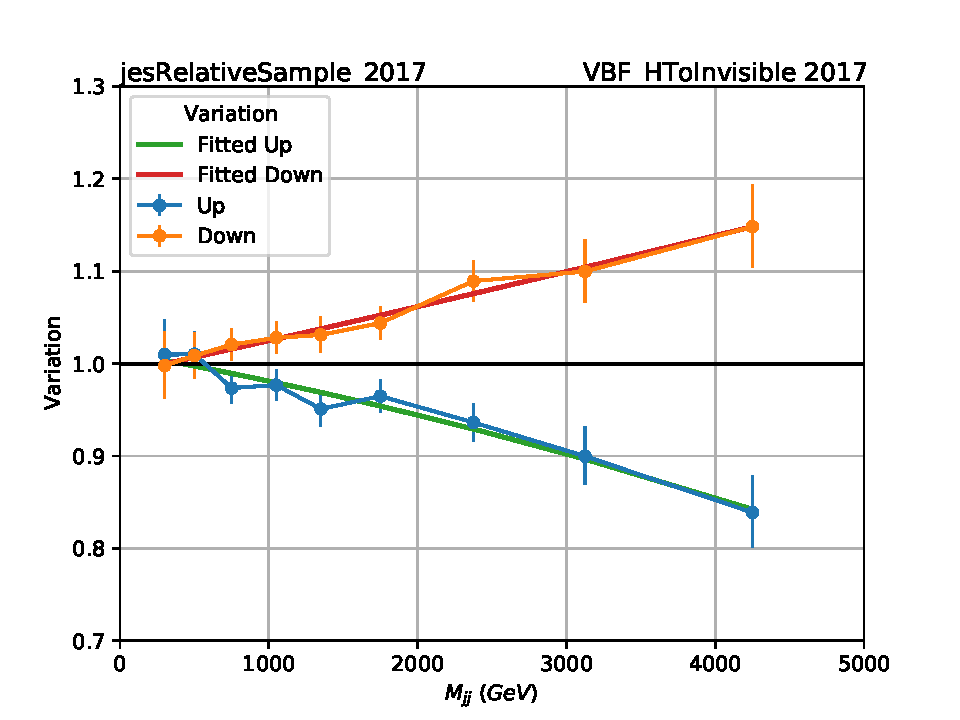
\includegraphics[width=0.49\textwidth]{ExperimentalUncertainties/JEC/VBF_HToInvisible_2017_jesRelativeSample_2017.pdf}
  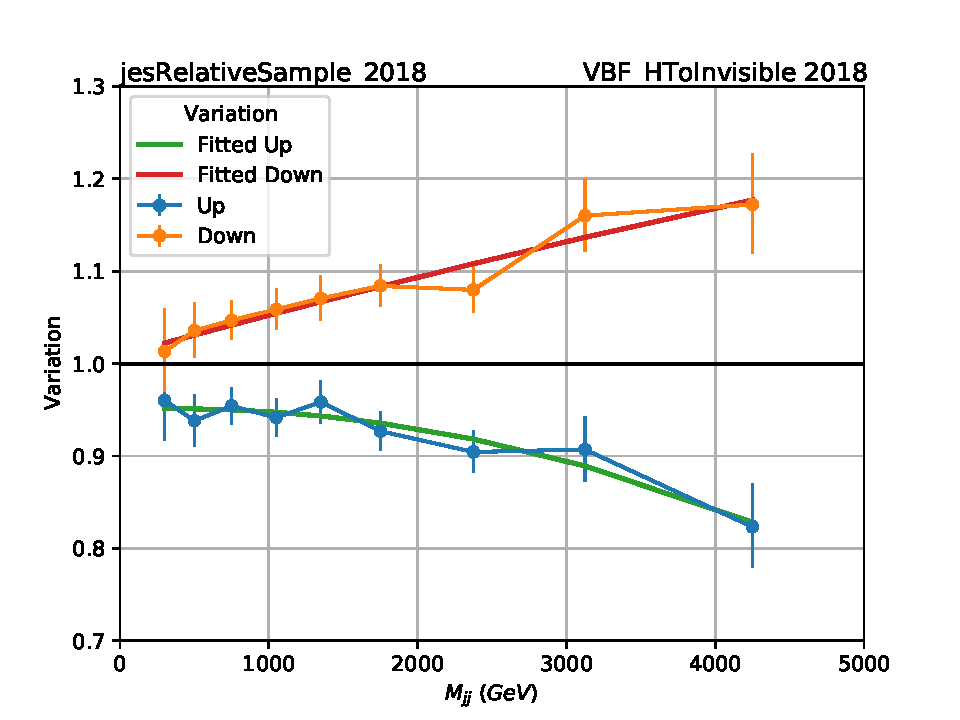
\includegraphics[width=0.49\textwidth]{ExperimentalUncertainties/JEC/VBF_HToInvisible_2018_jesRelativeSample_2018.pdf}
  \caption{Relative sample JEC uncertainties calculated with strong $\Zvvjets$ (top) and VBF $\hinv$ signal (bottom). Left column shows the 2017 results, 
  while the right column shows the 2018 results. The fitted uncertainties, shown in solid lines, are used as the final uncertainty shapes.}
  \label{fig:znunu_jec_uncs}
\end{figure}

As discussed in Sec.~\ref{subsubsec:hf_noise_est}, a $20\%$ flat uncertainty is applied to the data-driven HF noise estimate, to take residual differences between
data and expected background yields into account.

Uncertainties on trigger efficiency reweighting, as discussed in Sec.~\ref{subsec:trigger_eff_reweighting}, are also applied in the analysis. For the electron, photon and
$\ptmiss$ trigger reweightings, flat uncertainties are applied on the transfer factors. The magnitudes of the flat uncertainties are $1\%$, $1\%$ and $2\%$ respectively. 

List of all theoretical and experimental uncertainties on transfer factors are shown in Tab.~\ref{tab:systematics}, together with the transfer factors they are applied on,
and their magnitudes.

\begin{table*}[htbp]
  \centering
  \caption{Experimental and theoretical sources of systematic uncertainties in the $\Vjets$ transfer factors. 
  The second column highlights on which ratio specifically a given source of uncertainty acts. 
  The subscript SR (CR) refers to the process yield in the SR (corresponding CRs). The impact on $\mjj$ is given in the 3rd column, 
  either as a single value (if no dependence on $\mjj$ is observed) or as a range of impact on low to high $\mjj$ values.
  }
  \def\arraystretch{1.05}
  \cmsTable{
  \begin{tabular}{l l c}
     \hline
     Source of uncertainty & Ratios & Uncertainty vs. \mjj\\% [\cmsTabSkip] % & Impact on $\brhinv$\\ [\cmsTabSkip]
     \hline
     \multicolumn{3}{c}{Theoretical uncertainties} \\% [\cmsTabSkip]
     \hline
     Ren. scale $\Vjets$ (VBF)      & $Z_{\mathrm{SR}}/W_{\mathrm{SR}}$   & 5--10\%  \\
     Ren. scale $\Vjets$ (strong)   & $Z_{\mathrm{SR}}/W_{\mathrm{SR}}$   & 5--10\%  \\
     Fac. scale $\Vjets$ (VBF)      & $Z_{\mathrm{SR}}/W_{\mathrm{SR}}$   & 1.5\%   \\
     Fac. scale $\Vjets$ (strong)   & $Z_{\mathrm{SR}}/W_{\mathrm{SR}}$   & 1.3\%   \\
     PDF $\Vjets$ (VBF)             & $Z_{\mathrm{SR}}/W_{\mathrm{SR}}$   & 0\% \\
     PDF $\Vjets$ (strong)          & $Z_{\mathrm{SR}}/W_{\mathrm{SR}}$  & 0\% \\
     NLO EW corr. $\Vjets$ (strong) & $Z_{\mathrm{SR}}/W_{\mathrm{SR}}$ & 0.5\%   \\%[\cmsTabSkip]
     Ren. scale $\phojets$ (VBF)    & $Z_{\mathrm{SR}}/\gamma_{\mathrm{CR}}$   & 6--10\%  \\
     Ren. scale $\phojets$ (strong) & $Z_{\mathrm{SR}}/\gamma_{\mathrm{CR}}$  & 6--10\%  \\
     Fac. scale $\phojets$ (VBF)    & $Z_{\mathrm{SR}}/\gamma_{\mathrm{CR}}$   & 2.5\%   \\
     Fac. scale $\phojets$ (strong) & $Z_{\mathrm{SR}}/\gamma_{\mathrm{CR}}$  & 2.5\%   \\
     PDF $\phojets$ (VBF)           & $Z_{\mathrm{SR}}/\gamma_{\mathrm{CR}}$   & 2.5\% \\
     PDF $\phojets$ (strong)        & $Z_{\mathrm{SR}}/\gamma_{\mathrm{CR}}$  & 2.5\% \\
     NLO EW corr. $\phojets$        & $Z_{\mathrm{SR}}/\gamma_{\mathrm{CR}}$ & 3\%   \\%[\cmsTabSkip]

     \hline
     \multicolumn{3}{c}{Experimental uncertainties}  \\ %[\cmsTabSkip]
     \hline
     Electron reco. eff.       & $Z_{\mathrm{CR}}/Z_{\mathrm{SR}}$, $W_{\mathrm{CR}}/W_{\mathrm{SR}}$ & $\approx0.5\%$ (per lepton)  \\
     Electron id. eff.         & $Z_{\mathrm{CR}}/Z_{\mathrm{SR}}$, $W_{\mathrm{CR}}/W_{\mathrm{SR}}$ & $\approx1\%$ (per lepton) \\
     Muon id. eff.             & $Z_{\mathrm{CR}}/Z_{\mathrm{SR}}$, $W_{\mathrm{CR}}/W_{\mathrm{SR}}$ & $\approx0.5\%$ (per lepton)  \\
     Muon iso. eff.            & $Z_{\mathrm{CR}}/Z_{\mathrm{SR}}$, $W_{\mathrm{CR}}/W_{\mathrm{SR}}$ & $\approx0.1\%$ (per lepton)  \\
     Photon id. eff.           & $Z_{\mathrm{SR}}/\gamma$       & 5\% \\
     
     Electron veto (reco)      & $Z_{\mathrm{SR}}/W_{\mathrm{SR}}$, $W_{\mathrm{CR}}/W_{\mathrm{SR}}$ & $\approx1.5$ (1)\% for VBF (strong) \\
     Electron veto (id)        & $Z_{\mathrm{SR}}/W_{\mathrm{SR}}$, $W_{\mathrm{CR}}/W_{\mathrm{SR}}$ & $\approx2.5$ (2)\% for VBF (strong) \\
     Muon veto                 & $Z_{\mathrm{SR}}/W_{\mathrm{SR}}$, $W_{\mathrm{CR}}/W_{\mathrm{SR}}$ & $\approx0.5$\% \\
     $\tau_{h}$ veto           & $Z_{\mathrm{SR}}/W_{\mathrm{SR}}$, $W_{\mathrm{CR}}/W_{\mathrm{SR}}$ & $\approx1$\% \\

     Electron trigger          & $Z_{\mathrm{CR}}/Z_{\mathrm{SR}}$, $W_{\mathrm{CR}}/W_{\mathrm{SR}}$ & $\approx1\%$  \\
     \ptmiss trigger           & $Z_{\mathrm{CR}}/Z_{\mathrm{SR}}$, $W_{\mathrm{CR}}/W_{\mathrm{SR}}$ & $\approx2\%$  \\
     Photon  trigger           & $Z_{\mathrm{SR}}/\gamma$                           & 1\% \\
     \hline
     \multirow{4}{*}{JES}      & $Z_{\mathrm{SR}}/W_{\mathrm{SR}}$         & 1--2\% \\
                               & $W_{\mathrm{CR}}/W_{\mathrm{SR}}$                 & 1.0--1.5\%  \\
                               & $Z_{\mathrm{CR}}/Z_{\nu\nu}$   		& 1\% \\
                               & $Z_{\mathrm{SR}}/\gamma$	    	& 3\% \\\hline
     \multirow{4}{*}{JER}  	   & $Z_{\mathrm{SR}}/W_{\mathrm{SR}}$         & 1.0--2.5\%  \\ 
                               & $W_{\mathrm{CR}}/W_{\mathrm{SR}}$                & 1.0--1.5\% \\
                               & $Z_{\mathrm{CR}}/Z_{\mathrm{SR}}$		& 1\% \\
                               & $Z_{\mathrm{SR}}/\gamma$	    	& 1--4\%  \\
     \hline
  \end{tabular}
}
  \label{tab:systematics}
\end{table*}

\clearpage